\documentclass[11pt,a4paper]{article}

\usepackage[utf8]{inputenc}
\usepackage[T1]{fontenc}
\usepackage{amsmath,amssymb,amsthm}
\usepackage{mathtools}
\usepackage{booktabs}
\usepackage{hyperref}
\usepackage{geometry}
\usepackage{enumitem}
\usepackage{listings}
\usepackage{longtable}
\usepackage{textcomp}
\usepackage{array}
\usepackage{tikz}
\usetikzlibrary{arrows.meta,positioning,calc,shapes.geometric,automata}

\geometry{margin=1in}
\setcounter{tocdepth}{2}

\newtheorem{definition}{Definition}[section]
\newtheorem{principle}[definition]{Principle}
\newtheorem{theorem}[definition]{Theorem}
\newtheorem{proposition}[definition]{Proposition}
\newtheorem{invariant}[definition]{Invariant}
\newtheorem{remark}[definition]{Remark}

\lstset{
  basicstyle=\ttfamily\small,
  columns=fullflexible,
  keepspaces=true,
  xleftmargin=2em,
  aboveskip=0.5em,
  belowskip=0.5em,
  breaklines=true,
  breakatwhitespace=true
}

\title{Deferred Settlement on Cash Equities\\[6pt]
\large The Open Window Between Trade-Date Recognition and Settlement-Date Custody Movement\\[4pt]
\normalsize Companion Document to the Ledger Framework Specification}
\author{R.\ Delloye}
\date{April 2026 --- v1.0}

\begin{document}
\maketitle

\begin{abstract}
The Ledger framework~\cite{ledger} reduces post-trade activity to a single primitive: the atomic move of a quantity between wallets, governed by a conservation law that holds by construction. The framework is silent, however, on a fact peculiar to cash-equity markets: under the prevailing T+2 (and, for US equities since 28~May~2024, T+1) cycle, the economic event of buying or selling a share is separated from the custody event of receiving or delivering it by one or two business days. During that window the buyer is economically long without having received the security, and the seller is economically short of cash without having received it. The trading book, the risk system, and the regulator all need to know the position from $T$; the depot and the nostro do not move until $T+\text{ISD}$.

This document specifies how the Ledger represents that gap. The design is deliberately minimal. It adds two wallet classes (\texttt{cpty\_virtual} and \texttt{csd\_virtual}), one obligation row in the data layer's $L_{15}$ leaf, and one workflow per obligation. It introduces \emph{zero} new fields on \texttt{PositionState}, \emph{no} fourth StatesHome map, \emph{no} new conservation carve-out, and \emph{no} new coordinate on the Generalised Position Model. The settlement window becomes a parameter of the standard machinery, not a doctrine of its own; T+0 atomic settlement on a distributed ledger and T+5 cross-border fail both fall out of the same construction. We build the design from scratch, demolish two naive alternatives along the way, walk through a standard buy and a standard sell at the level of individual moves with conservation verified at each step, extend the construction to seven variants and three composition cases, prove a Conservation Lifting Theorem that subsumes the open-window invariant, give a CDM cross-walk identifying five strategic gaps, and close with a list of nineteen invariants ($\mathrm{DS1}$ through $\mathrm{DS19}$) that an implementation must satisfy. The discipline of the document is pedagogical: a reader who stops after Section~\ref{sec:standard-buy} has a working mental model; the remaining sections add complexity one variant at a time, each motivated by a case the simpler model could not handle.
\end{abstract}

\tableofcontents
\clearpage

%==============================================================================
\section{The Problem}
\label{sec:problem}
%==============================================================================

\subsection{The economic fact and the custody fact diverge}

Equity markets settle on a delay. When a portfolio manager places a buy order on the New York Stock Exchange and that order is matched at $14{:}32{:}11$~UTC on Monday, the trade is \emph{economically} done in the same instant: the manager has acquired exposure to the share's price, owes cash, and is entitled to dividends declared on or after that timestamp. The custody event --- the actual transfer of the share into the buyer's depot account at the central securities depository (CSD) and the corresponding debit of the buyer's cash nostro --- does not occur until Wednesday, the following day, or sometimes Thursday in cross-border cases. Between Monday and Wednesday the buyer sits in a state that no scalar wallet balance can cleanly describe: long the security in the eyes of the trading book, the risk system, the accounting standard, and the regulator; flat in the eyes of the CSD and the cash agent.

We will call this interval the \emph{open settlement window}, denote it $[T, t_d]$ where $T$ is trade-execution time and $t_d$ is intended settlement date, and call its duration the \emph{settlement cycle}. For US cash equities since 28~May~2024 the cycle is one business day (T+1); for EU and UK cash equities until at least 11~October~2027 it is two (T+2); for some Asian markets and atomic distributed-ledger settlement venues it is zero (T+0); for cross-border fails it can extend to five business days or more before regulatory buy-in is mandated. The duration is a parameter; the structural fact --- that economic recognition and custody movement do not coincide --- is universal.

\subsection{A first concrete case}

To make the divergence quantitative, consider a single trade, executed in clean conditions, with no failures or corrections.

\begin{itemize}[nosep]
\item \textbf{Date of execution.} $T = 2026\textnormal{-}04\textnormal{-}30$, $14{:}32{:}11$~UTC. The market is XNYS; the settlement cycle is T+2.
\item \textbf{Intended settlement date.} $t_d = 2026\textnormal{-}05\textnormal{-}04$.
\item \textbf{Trade.} Our portfolio (real wallet $w_{\mathrm{us}}$) buys 100 shares of \texttt{XYZ} at \$50.00 per share. The cash leg is \$5{,}000.00; the counterparty is the broker Goldman Sachs (LEI \texttt{784F5XWPLTWKTBV3E584}, denoted hereafter $\mathrm{GS}$).
\item \textbf{Pre-trade state.} $w_{\mathrm{us}}.\mathrm{own}(\mathrm{USD}) = 1{,}000{,}000.00$ and $w_{\mathrm{us}}.\mathrm{own}(\mathrm{XYZ}) = 0$. The custodian's daily cash statement (an ISO~20022 \texttt{camt.053}) reports our nostro balance as \$1{,}000{,}000.00.
\item \textbf{Mark-to-market.} \texttt{XYZ} closes at \$50.00 on Monday, \$52.00 on Tuesday (T+1), and \$51.50 on Wednesday (T+2).
\end{itemize}

The question is: \emph{what does the Ledger know on Tuesday at the close of business?} On Monday no shares have arrived; no cash has left. On Tuesday no shares have arrived; no cash has left. The custodian's nostro statement still shows \$1{,}000{,}000.00; the depot statement still shows zero \texttt{XYZ}. By any reading of the \emph{custody} record, nothing has happened.

But our trading book has a position of $+100$ \texttt{XYZ} at $T$ marked to \$52.00 on Tuesday close, against a liability to pay \$5{,}000.00 to $\mathrm{GS}$ on Wednesday. The portfolio's value has moved from \$1{,}000{,}000.00 on Monday morning to:
\[
V_{T+1} \;=\; 100 \cdot 52.00 \;+\; \underbrace{(1{,}000{,}000.00 - 5{,}000.00)}_{\text{cash net of payable}} \;=\; 5{,}200.00 + 995{,}000.00 \;=\; 1{,}000{,}200.00,
\]
giving a profit-and-loss number of $+\$200.00$ on Tuesday close, with \emph{zero cash movement} and \emph{zero custody movement}. This is the headline fact of trade-date accounting: the \$200 is real, recognised under IFRS~9 paragraph B3.1.3 (the regular-way exception) and ASC~320-10-25-3, and it is reflected in the firm's regulatory capital, daily VaR, and overnight risk reports. It is also a number that no system limited to scalar wallet balances over real custody accounts can produce, because there is nothing on those accounts that has changed.

\subsection{What the Ledger must do}

The Ledger has six obligations during the open window. The design of this document is the smallest extension that satisfies all six simultaneously.

\begin{enumerate}[nosep]
\item \textbf{Recognise the economic position at $T$.} The portfolio is long $100$ \texttt{XYZ} from $14{:}32{:}11$~UTC on Monday. Mark-to-market PnL flows from $T$, not from $t_d$.
\item \textbf{Carry the per-counterparty obligation.} The buyer owes \$5{,}000.00 to $\mathrm{GS}$; $\mathrm{GS}$ owes 100 \texttt{XYZ} to the buyer. These claims are net-settleable, ageing, capital-bearing, and counterparty-keyed. They must be observable as quantities, not just narratively.
\item \textbf{Reconcile to the external nostro and depot.} The custodian's \texttt{camt.053} and the CSD's depot statement remain authoritative for what is \emph{at} the custodian and \emph{at} the CSD. The Ledger must satisfy an algebraic identity with those statements at every wall-clock $t$, every business day, including during the open window.
\item \textbf{Register the legal duty.} A settlement obligation is a legal artefact governed by the master agreement, the CSD rulebook, and (in the EU) the CSDR fails regime. It has a deadline, a discharge predicate, a failure-handler, and a penalty clock. It must be a first-class object, not an attribute scattered across log lines.
\item \textbf{Discharge only on witness.} A move from \emph{open} to \emph{settled} is admitted only when an attested external observation arrives: a CSD finality message (\texttt{sese.025}), a custodian cash-credit advice (\texttt{camt.054}), or a multi-source quorum when those are silent. No clock-driven auto-discharge. No optimistic discharge. Silence is itself attested before any state change.
\item \textbf{Preserve replay determinism.} The witness substream is consumed in deterministic order; restated finality, partial credits, wire recalls, and out-of-order arrivals all converge to the same terminal state. This is the property that lets the Ledger time-travel and the property that lets a deterministic reference interpreter substitute for the production runtime in tests.
\end{enumerate}

\subsection{Document discipline}

We will build the design move-by-move. After this section, we will demolish two strawmen (Section~\ref{sec:strawmen}), define the state model (Section~\ref{sec:state-model}), walk through the canonical buy with conservation verified at every step (Section~\ref{sec:standard-buy}), do the same for the sell (Section~\ref{sec:standard-sell}), then add variants and composition cases (Section~\ref{sec:variants}, Section~\ref{sec:composition}), reconcile to the nostro (Section~\ref{sec:reconciliation}), state the accounting and regulatory footprint (Section~\ref{sec:accounting}), provide the CDM cross-walk (Section~\ref{sec:cdm}), give implementation notes (Section~\ref{sec:implementation}), declare what is out of scope (Section~\ref{sec:out-of-scope}), and close with a glossary (Section~\ref{sec:glossary}). Throughout, every claim is concrete: every PnL number is computed in the document, every conservation table sums to zero in print, every invariant is stated in a numbered block, and every workflow is specified with its trigger, body, and termination condition.

\clearpage
%==============================================================================
\section{Why the Naive Solutions Fail}
\label{sec:strawmen}
%==============================================================================

Before describing the design, we describe two natural-looking alternatives and demonstrate that each violates one of the six requirements above. The exercise is not pedantic: each strawman embodies a misconception we have seen in production systems, and each demolition surfaces a structural requirement that the eventual design must satisfy.

\subsection{Strawman 1: ``Debit the nostro at T''}
\label{sec:strawman-1}

\textbf{The proposal.} On trade execution at $T$, atomically debit the cash nostro wallet by \$5{,}000.00 and credit the depot wallet by 100 \texttt{XYZ}. Treat the trade like an instantaneous settlement and reconcile to the custodian later.

\textbf{The appeal.} It is the simplest thing one can do on a single-primitive ledger: one move pair, one transaction, conservation holds atomically, no new state. The economic position is recognised at $T$ (good); the per-counterparty obligation is implicit in the move (it was sourced from $\mathrm{GS}$, registered in the metadata, fine); the legal duty becomes the move itself.

\textbf{What breaks.} The custodian's daily \texttt{camt.053} statement, sent at end of day Monday, will report a nostro balance of \$1{,}000{,}000.00. Our internal record will say \$995{,}000.00. The reconciliation fails. There are now two diverging stories about the same cash account:
\begin{itemize}[nosep]
\item \textbf{Internal:} ``We paid for the share. The cash is gone.''
\item \textbf{External:} ``Your account holds \$1{,}000{,}000.00. Nothing has been debited.''
\end{itemize}

The break is exactly \$5{,}000.00 every day for two days, with no operational meaning. This is not a transient anomaly; it is the system in normal working order. To resolve it, the operations team must invent a category called ``cash in transit'' and explain why it is sometimes a real liability (when the wire has been sent) and sometimes a fictional one (when it has not). Worse, on Wednesday morning when the nostro \emph{is} actually debited by \$5{,}000.00 via the cash agent, the Ledger has nothing to apply that movement to: its internal state has already been reduced. Either the Wednesday \texttt{camt.054} cash-debit advice is treated as a no-op (in which case we have lost a piece of evidence the auditor will demand to see) or it is applied a second time (in which case \$5{,}000.00 disappears).

\textbf{The deeper failure.} The strawman \emph{conflates two distinct facts}: the economic fact (that we now own the share from $T$) and the custody fact (that the cash actually leaves the nostro at $t_d$). They are different events, attested by different sources, on different business days, with different legal consequences. A ledger that collapses them loses information the framework cannot recover.

\textbf{Requirement extracted.} The economic move at $T$ and the custody move at $t_d$ must be \emph{separately observable} and \emph{separately attested}. They cannot share a single move-pair.

\subsection{Strawman 2: ``Recognise nothing until T+2''}
\label{sec:strawman-2}

\textbf{The proposal.} At $T$, record the trade as metadata only: a row in some pending-trades log. Make no moves. Wait until the CSD's \texttt{sese.025} arrives on Wednesday, then emit the move pair (depot $+100$ \texttt{XYZ}, nostro $-\$5{,}000.00$). The Ledger matches the external record at every instant.

\textbf{The appeal.} The ledger never disagrees with the custodian. Reconciliation is trivial. There is nothing to ``unwind'' on a fail; if Wednesday's message never arrives, no moves were ever made.

\textbf{What breaks.} On Tuesday close at \$52.00, the trading book asks the Ledger: ``what is our P\&L?'' The Ledger responds: ``You hold zero \texttt{XYZ}. Your cash is \$1{,}000{,}000.00. P\&L is zero.'' This is wrong. The portfolio manager has \$200.00 of fair-value gain on the position they have already acquired. Under IFRS~9.B3.1.3 and ASC~320-10-25-3, a regular-way trade is recognised at trade date for fair-value-through-profit-or-loss instruments; settlement-date recognition is a banking-book exception that does \emph{not} apply to a dealer trading book. The CRR Article 325 (FRTB) and Article 274 (SA-CCR) capital calculations \emph{require} trade-date positions; a bank that uses settlement-date positions for its capital reports has misstated its capital.

The strawman is also operationally broken on the upstream side. The risk engine wants the position from $14{:}32{:}11$~UTC on Monday for its overnight VaR; the trader's P\&L blotter wants it for the daily mark; the regulatory transaction report (MiFIR Article~26 / RTS~22) is due at $23{:}59$ Monday local time of the relevant national competent authority and must contain $T$, not $t_d$. None of these consumers can wait until Wednesday.

\textbf{The deeper failure.} The strawman \emph{subordinates the economic record to the custody record}. The custody record is an attestation about a particular external book on a particular calendar; it is not the source of truth about who owns the position. The buyer owns the position from $T$ regardless of what the CSD or the cash agent has done. A ledger that refuses to recognise that fact has chosen the wrong system of record.

\textbf{Requirement extracted.} The economic position must be \emph{observable from $T$} on the trading book's wallet, by every consumer (risk, capital, regulatory, accounting), without waiting for or being conditional on the custody event.

\subsection{The intersection of the two requirements}

The two demolitions, taken together, give us the shape of the design.

\begin{itemize}[nosep]
\item From Strawman~1: the cash and securities cannot \emph{actually} move on the trading book's nostro and depot wallets at $T$; those wallets must remain consistent with the external records, which do not change until $t_d$.
\item From Strawman~2: the economic position \emph{must} be reflected on the trading book at $T$; there is no consumer for whom waiting is acceptable.
\end{itemize}

The only construction that satisfies both is one in which the trade-date move \emph{recognises the economic position} (changes the trading book's view of what it owns) but the corresponding contra balance is held on a wallet that is \emph{not} the external nostro or depot. The contra is per-counterparty, signed (because the same trade simultaneously creates a payable on cash and a receivable on the security), and explicitly distinct from the wallets that mirror external custody. The custody-date move at $t_d$ then drains the contra into a separate wallet class that mirrors the external book at finality.

The next section makes this construction precise.

\clearpage
%==============================================================================
\section{The State Model}
\label{sec:state-model}
%==============================================================================

The construction we settled on adds three things to the Ledger: two new \emph{wallet classes}, one new \emph{obligation row} in the existing data-layer leaf $L_{15}$ (the data-spec \texttt{Obligation} leaf), and a \emph{lifecycle finite-state machine} attached to that obligation row. It adds nothing to \texttt{PositionState}, nothing to \texttt{UnitStatus}, nothing to \texttt{ProductTerms}, no fourth StatesHome map, no new GPM coordinate, and no new conservation carve-out. The conservation law $\sum_{w \in \mathcal{W}} w_t(u) = 0$ holds over a constant universe $\mathcal{W}$ that grows by the new wallets but admits the new wallets as ordinary participants.

\subsection{The triple}

A deferred-settlement obligation is represented by three coordinated artefacts. The triple is the canonical mental model; everything else follows from it.

\begin{definition}[Deferred-settlement triple]
\label{def:triple}
A trade $\tau$ that opens a settlement window of duration $t_d - T$ produces three coordinated artefacts on the Ledger:
\begin{enumerate}[nosep]
\item \textbf{A real-wallet \texttt{own} write at $T$.} The trading book's real wallet $w_{\mathrm{real}}$ has its $\mathrm{own}$ coordinate updated by the standard v10.3 move algebra. This recognises the economic position. It is performed exactly once, at $T$, by the \texttt{apply\_trade\_move} handler. It is \emph{never} reversed by any settlement event.
\item \textbf{A \texttt{cpty\_virtual} contra balance.} For each $(w_{\mathrm{real}}, \text{cpty\_lei}, u)$ triple, a single virtual wallet $w_{\mathrm{PS}}[w_{\mathrm{real}}, \text{cpty}, u]$ holds the per-counterparty open-obligation quantity. Its sign carries the side: positive means we owe; negative means they owe us. It is debited or credited at $T$ atomically with the real-wallet move, and drained at $t_d$ when finality is attested.
\item \textbf{An $L_{15}.\mathrm{Obligation}$ row.} A row in the data-layer's $L_{15}$ leaf, kind \texttt{SettlementInstructionDelivery}, carrying the obligation's lifecycle state, intended settlement date, discharge predicate, CSDR clock, and audit chain. It is created at $T$, advanced by witness arrival, and reaches a terminal state at or after $t_d$.
\end{enumerate}
\end{definition}

The division of labour is sharp. The \texttt{cpty\_virtual} pair holds the \emph{contra-quantity}; the $L_{15}$ row holds the \emph{lifecycle}. There is no transaction-level FSM in storage --- the trade-level status (\texttt{Settled}, \texttt{InFlight}, \texttt{PartiallySettled}, \ldots) is a pure projection function over the per-leg $L_{15}$ rows, computed on read. We define this projection in Section~\ref{sec:lifecycle-projection}.

\subsection{Wallet classes}

\begin{definition}[Wallet classes]
\label{def:wallet-classes}
Every wallet in $\mathcal{W}$ belongs to exactly one of four classes, recorded as a sidecar field on the $\mathrm{WalletRegistry}$:
\begin{description}[style=nextline,leftmargin=1.5em]
\item[\texttt{real}] A book-of-record wallet whose \texttt{own} coordinate represents an economic position the firm holds. Examples: $w_{\mathrm{us}}$ (the firm's portfolio), $w_{\mathrm{book42}}$ (a particular trading book). Real wallets are written at $T$ by \texttt{apply\_trade\_move} and never moved by settlement.
\item[\texttt{cpty\_virtual}] A per-counterparty virtual wallet keyed $(w_{\mathrm{real}}, \text{cpty\_lei}, u)$, holding the open-window contra-quantity for that real wallet against that counterparty for that unit. Surface forms: $w_{\mathrm{PS}}[w_{\mathrm{real}}, \mathrm{cpty}, \mathrm{ccy}]$ for cash-leg obligations, $w_{\mathrm{PSS}}[w_{\mathrm{real}}, \mathrm{cpty}, \mathrm{ISIN}]$ for securities-leg obligations. Both surface forms are instances of the same wallet class.
\item[\texttt{csd\_virtual}] A mirror wallet that represents the position of an external holder at a CSD or correspondent bank, keyed $(\mathrm{csd\_or\_bank\_lei}, \mathrm{holder\_lei}, u)$. Surface forms: $w_{\mathrm{DTC\_depot\_mirror}}[\text{holder}]$, $w_{\mathrm{JPMC\_nostro\_mirror}}[\text{holder}]$. \texttt{csd\_virtual} wallets absorb the contra at finality, mirroring what the external book records.
\item[\texttt{inception}] The singleton genesis wallet $w_{\mathrm{genesis\_inception}}$ that establishes the absolute baseline of the constant universe per v10.3 \S2.7's inception-move discipline. Every pre-trade real-wallet balance has a corresponding equal-and-opposite entry on $w_{\mathrm{genesis\_inception}}$ so that the absolute form of conservation $\sum_{w \in \mathcal{W}} w_t(u) = 0$ holds from the first state. The inception wallet is written exactly once per unit at registry creation and is never moved thereafter; it is omitted from per-state delta tables in worked examples (because $\Delta = 0$) but is part of $\mathcal{W}$.
\end{description}
\end{definition}

\begin{remark}[Side is sign, not class]
Earlier drafts of this design carried a four-class taxonomy with \texttt{cpty\_virtual\_payable} and \texttt{cpty\_virtual\_receivable} as separate classes. We collapsed them: the \emph{side} of an obligation (do we owe, or do they owe us?) is encoded as the sign of the stored balance, not as a wallet class. A positive balance on $w_{\mathrm{PS}}[w_{\mathrm{us}}, \mathrm{GS}, \mathrm{USD}]$ means we owe GS USD; a negative balance means GS owes us USD. Disclosure-layer gross numbers, when required by IFRS~7 paragraph 13C, are projections:
\begin{align*}
\mathrm{gross\_payable}[w, \mathrm{cpty}, u]   &\;=\; \max(0, w_{\mathrm{PS}}[w, \mathrm{cpty}, u].\mathrm{own}), \\
\mathrm{gross\_receivable}[w, \mathrm{cpty}, u] &\;=\; \max(0, -w_{\mathrm{PS}}[w, \mathrm{cpty}, u].\mathrm{own}).
\end{align*}
Storage is signed; disclosure is gross by projection. This eliminates a class enum that would otherwise leak through the type system.
\end{remark}

\subsection{Sidecar metadata on \texttt{WalletRegistry}}

The new wallet classes induce sidecar columns on the \texttt{WalletRegistry}, none of which are state. They are KYC-style metadata that resolve at registry creation and do not vary with transactions:

\begin{lstlisting}
WalletRegistry sidecar columns:
  wallet_class             : { real | cpty_virtual | csd_virtual | inception }
  real_wallet              : FK to the owning real wallet
                             (NULL for real wallets and csd_virtual)
  cpty_lei                 : LEI of the counterparty
                             (NULL if not counterparty-keyed)
  csd_lei                  : LEI of the CSD or correspondent bank
                             (NULL unless csd_virtual)
  holder_lei               : LEI of whose mirror this is
                             (NULL unless csd_virtual)
  expected_settle_window   : { T+0 | T+1 | T+2 | T+3 } per venue convention
\end{lstlisting}

The crucial point is that \emph{no field is added to \texttt{PositionState}}. Both \texttt{cpty\_virtual} and \texttt{csd\_virtual} balances live in the same \texttt{PositionState[wallet, unit]} table that holds real-wallet balances, on the same \texttt{own} coordinate. The new wallets are ordinary rows in $\mathrm{WalletRegistry}$; their balances are ordinary rows in $\mathrm{PositionState}$. The framework's existing scan-by-wallet, project-on-read, conservation-by-construction machinery applies uniformly.

\subsection{StatesHome compliance}

The design is constrained by the v10.3 StatesHome principle: every piece of state lives in exactly one of the three maps (\texttt{ProductTerms}, \texttt{UnitStatus}, \texttt{PositionState}) plus the \texttt{WalletRegistry}. The deferred-settlement extension touches only $\mathrm{PositionState}$ (via new wallet rows on the existing $\mathrm{own}$ coordinate) and $\mathrm{WalletRegistry}$ (via the sidecar columns above). It does not add a fourth map. Table~\ref{tab:stateshome} records the explicit check.

\begin{table}[h]
\centering
\begin{tabular}{lll}
\toprule
\textbf{StatesHome map} & \textbf{Touched?} & \textbf{How?} \\
\midrule
$\mathrm{ProductTerms}[u]$       & no  & cash and security terms unchanged \\
$\mathrm{UnitStatus}[u]$         & no  & instrument-level lifecycle unaffected \\
$\mathrm{PositionState}[w, u]$   & yes & only via existing handlers; only on \texttt{own} \\
$\mathrm{WalletRegistry}[w]$     & yes & sidecar metadata (3 classes) \\
\bottomrule
\end{tabular}
\caption{StatesHome conformance check.}
\label{tab:stateshome}
\end{table}

The lifecycle FSM lives on the $L_{15}.\mathrm{Obligation}$ row, which is part of the data layer's smart-contract execution data, not StatesHome. This is the right home: $L_{15}$ is exactly the leaf the data spec reserves for canonical obligation records.

\subsection{The constant universe and conservation}

\begin{definition}[Constant universe]
\label{def:universe}
$\mathcal{W} = \mathcal{W}_{\mathrm{real}} \cup \mathcal{W}_{\mathrm{cpty\_virtual}} \cup \mathcal{W}_{\mathrm{csd\_virtual}} \cup \mathcal{W}_{\mathrm{inception}}$ is the \emph{constant} wallet universe over which conservation is asserted. ``Constant'' here means: the same set of wallet identifiers at every wall-clock $t$; new wallets enter the universe at a defined zero balance for every unit.
\end{definition}

\begin{invariant}[Conservation over $\mathcal{W}$]
\label{inv:conservation}
For every unit $u$ and every wall-clock $t$,
\[
\sum_{w \in \mathcal{W}} w_t(u) \;=\; 0.
\]
The sum runs over all real, cpty\_virtual, csd\_virtual, and inception wallets in the universe. The invariant admits no carve-out for state-only transactions (which contribute zero to every wallet sum) or for finality (whose move pair sums to zero). Section~\ref{sec:conservation-lifting} proves this as a corollary of the Conservation Lifting Theorem with five named hypotheses.
\end{invariant}

\subsection{The lifecycle FSM}
\label{sec:lifecycle-fsm}

The legal duty associated with each obligation row is a finite-state machine. We give the closed-sum specification first; the transition rules and witness discipline follow.

\begin{definition}[Lifecycle states]
\label{def:lifecycle-states}
The lifecycle of an $L_{15}.\mathrm{Obligation}$ row is described by a state $\sigma(o) \in \mathcal{L}$, where $\mathcal{L}$ is the closed sum:
\[
\mathcal{L} \;=\; \{\,\mathtt{Pending},\; \mathtt{Instructed},\; \mathtt{PartiallySettled},\; \mathtt{Discharged},\; \mathtt{Failed}(r),\; \mathtt{BoughtIn},\; \mathtt{Cancelled},\; \mathtt{Compensated}\,\}
\]
where $r$ ranges over a closed-sum \texttt{FailureReason}. The terminal set is $F_{\mathrm{terminal}} = \{\mathtt{Discharged}, \mathtt{Cancelled}, \mathtt{BoughtIn}, \mathtt{Compensated}\}$. \texttt{Failed} is terminal-conditional: it admits transitions to \texttt{BoughtIn} or \texttt{Compensated} via the CSDR resolution path; otherwise it is absorbing.
\end{definition}

\begin{lstlisting}
type LifecycleState =
  | Pending             (* registered at T; awaiting instruction emission   *)
  | Instructed          (* sese.023 dispatched; awaiting CSD finality       *)
  | PartiallySettled    (* partial discharge witnessed; residual still open *)
  | Discharged          (* terminal: full witness-driven discharge          *)
  | Failed of FailureReason
                        (* terminal-conditional: deadline missed or fail
                           message; admits BuyIn or Compensated             *)
  | BoughtIn            (* terminal: CSDR mandatory buy-in resolved         *)
  | Cancelled           (* terminal: pre-instruction four-eyes CORRECTION   *)
  | Compensated         (* terminal: cash-in-lieu, close-out, manual override *)

type FailureReason =
  | DeadlineMissed
  | NoCover                       (* securities short for delivery   *)
  | NoFunds                       (* cash short for payment          *)
  | CounterpartyDefault of LEI
  | CsdReject of CsdRejectCode    (* normalised closed sum           *)
  | LegInconsistent of WhichLeg   (* DvP partial-fail asymmetry      *)
  | Manual of OperatorId
\end{lstlisting}

The allowed transitions are:
\begin{align*}
\mathtt{Pending}      &\;\to\; \mathtt{Instructed}                                  \quad\text{(\texttt{sese.023} dispatch witness)} \\
\mathtt{Pending}      &\;\to\; \mathtt{Cancelled}                                   \quad\text{(four-eyes pre-instruction CORRECTION)} \\
\mathtt{Instructed}   &\;\to\; \mathtt{PartiallySettled} \mid \mathtt{Discharged} \mid \mathtt{Failed}(r) \quad\text{(witness)} \\
\mathtt{PartiallySettled} &\;\to\; \mathtt{Discharged} \mid \mathtt{Failed}(r)      \quad\text{(witness on residual)} \\
\mathtt{Failed}(r)    &\;\to\; \mathtt{BoughtIn} \mid \mathtt{Compensated}          \quad\text{(CSDR resolution path)} \\
\sigma                &\;\to\; \mathtt{Compensated}                                 \quad\text{(four-eyes manual override; }\sigma \notin F_{\mathrm{terminal}}\text{)}.
\end{align*}

All other transitions are forbidden by the closed-sum constraint. Compile-time enforcement is via exhaustive pattern match on \texttt{LifecycleState} in the step function (Section~\ref{sec:implementation}). Figure~\ref{fig:fsm} draws the transitions.

\begin{figure}[h]
\centering
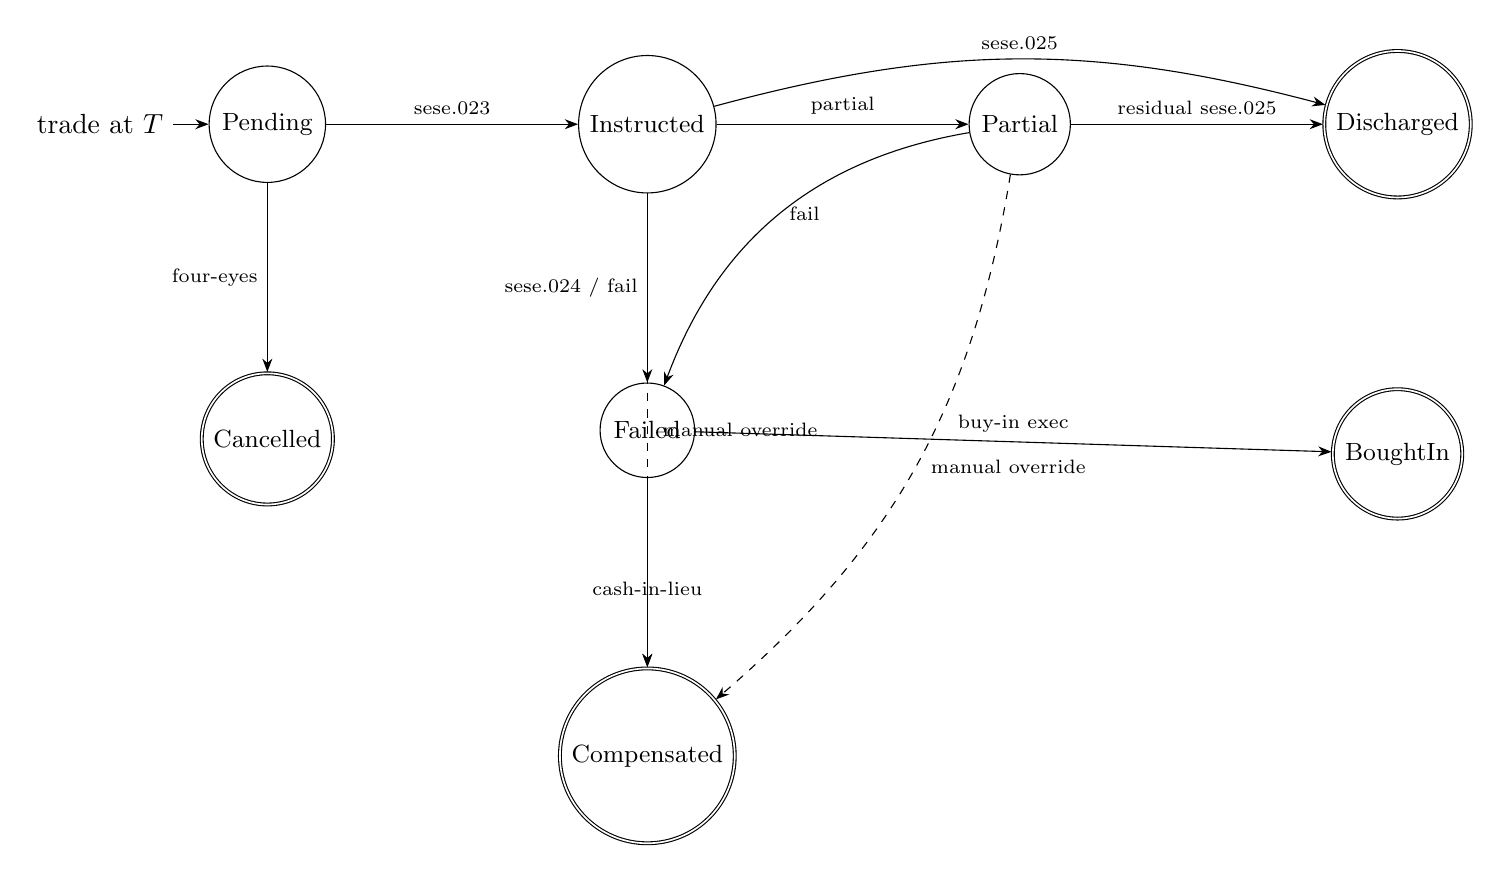
\begin{tikzpicture}[->,>=Stealth,node distance=2.4cm and 3.2cm,
                    every state/.style={font=\small, minimum size=1.2cm}]
  \node[state, initial, initial text={trade at $T$}] (P)  {Pending};
  \node[state, right=of P]                            (I)  {Instructed};
  \node[state, right=of I]                            (PS) {Partial};
  \node[state, accepting, right=of PS]                (D)  {Discharged};
  \node[state, below=of I]                            (F)  {Failed};
  \node[state, accepting, below=of D]                 (BI) {BoughtIn};
  \node[state, accepting, below=of P]                 (C)  {Cancelled};
  \node[state, accepting, below=of F]                 (CO) {Compensated};
  \path
    (P)  edge node[above]{\scriptsize sese.023}        (I)
    (P)  edge node[left] {\scriptsize four-eyes}        (C)
    (I)  edge node[above]{\scriptsize partial}          (PS)
    (I)  edge[bend left=15] node[above]{\scriptsize sese.025} (D)
    (I)  edge node[left] {\scriptsize sese.024 / fail}  (F)
    (PS) edge node[above]{\scriptsize residual sese.025}(D)
    (PS) edge[bend right] node[right]{\scriptsize fail}  (F)
    (F)  edge node[above]{\scriptsize buy-in exec}      (BI)
    (F)  edge node[below]{\scriptsize cash-in-lieu}     (CO)
    (PS) edge[dashed,bend left=20] node[right,xshift=2pt]{\scriptsize manual override} (CO)
    (I)  edge[dashed] node[right,xshift=2pt]{\scriptsize manual override} (CO);
\end{tikzpicture}
\caption{The lifecycle FSM. Solid arrows are witness-driven transitions; dashed arrows are four-eyes manual overrides. Accepting states are the terminal set $F_{\mathrm{terminal}} = \{\mathtt{Discharged}, \mathtt{BoughtIn}, \mathtt{Cancelled}, \mathtt{Compensated}\}$. \texttt{Failed} is terminal-conditional.}
\label{fig:fsm}
\end{figure}

\subsection{Transaction-level status as a projection}
\label{sec:lifecycle-projection}

A typical DvP cash-equity trade has \emph{two} obligation rows: one for the securities leg ($o_{\mathrm{sec}}$) and one for the cash leg ($o_{\mathrm{cash}}$). They are independent in the FSM; each is transitioned by its own witness. There is, however, a useful trade-level question: ``has this trade settled in full?'' The Ledger answers it not with a stored field but with a pure projection function over the leg states.

\begin{lstlisting}
def tx_status(tx: Transaction) -> TransactionView:
    legs = [o for o in L_15 if o.tx_id == tx.tx_id]
    states = {o.state for o in legs}
    if all(s == Discharged for s in states):                          return Settled
    if any(s == Compensated for s in states) and rest_terminal:       return Compensated
    if any(s == Cancelled   for s in states) and rest_terminal:       return Cancelled
    if any(s == PartiallySettled for s in states):                    return PartiallySettled
    if any(s == Failed for s in states) and rest_terminal:            return Failed
    if all(s == Instructed for s in states):                          return Instructed
    if all(s in {Pending, Instructed} for s in states):               return InFlight
    return Mixed   # leg-inconsistent; spawn wf-confirm-break

class TransactionView = Settled | Compensated | Cancelled | PartiallySettled
                       | Failed | Instructed | InFlight | Mixed
\end{lstlisting}

The function is pure, total over the input domain, and \texttt{Mixed} is the well-defined return for a leg-inconsistent state (one leg \texttt{Discharged}, the other \texttt{Failed}) which spawns a \texttt{wf-confirm-break} workflow. Operational queues that need to filter on transaction-level status use a materialised view computed by the same projection at write time and indexed; the eventual-consistency window is sub-second.

The reason \texttt{tx\_status} is a projection rather than a stored field is structural. Storing it would create a second source of truth for trade-level state, vulnerable to the very class of reconciliation failure the framework is designed to eliminate. Computing it forces the per-leg states to remain canonical and the trade-level view to remain dependent --- which is the architecturally correct relationship.

\subsection{Witness-driven discharge}
\label{sec:witness-driven}

The single most important rule of the lifecycle is that no transition out of \texttt{Pending} (other than four-eyes \texttt{Cancelled}) occurs without a verified witness.

\begin{principle}[Witness-driven discharge]
\label{prin:witness}
An obligation $o$ transitions to a non-\texttt{Pending}, non-\texttt{Cancelled} state if and only if:
\begin{enumerate}[nosep]
\item An \emph{attestation envelope} (defined in Section~\ref{sec:envelope}) has been recorded on the data layer's external-confirmation leaf $L_{11}$ (the data-spec \texttt{ExternalConfirmation} leaf);
\item The envelope's signature, schema, and dedup-key have been verified, and (where required by the multi-source policy) the envelope is corroborated by a quorum of independent sources;
\item The envelope's payload reconciles with the obligation's discharge predicate within the per-currency tolerance pinned in $L_7^{\mathrm{P}}$ (the data-spec \texttt{PolicyConfiguration} sidecar).
\end{enumerate}
The framework \emph{never} marks a leg \texttt{Discharged} by inference, by clock, or by absence of evidence. Watchdog timers trigger a break workflow, not an auto-fail (Section~\ref{sec:absence-of-finality}).
\end{principle}

The principle is non-trivial. A naive workflow would say: ``if no fail message has arrived by $t_d + 0.5$~bd, mark the obligation \texttt{Discharged} optimistically.'' This is wrong on two counts: it admits silence as evidence, and it makes the ledger's state a function of clocks rather than of evidence. The framework's discipline is that silence is itself attested --- a \texttt{silence\_attestation} envelope is generated by the watchdog, recorded on $L_{11}$, and used to open a break workflow that escalates for human action --- but the underlying obligation \emph{remains} in \texttt{Pending} or \texttt{Instructed} until a positive witness arrives or a four-eyes correction transitions it explicitly. This is what makes the ledger time-travellable: the state at any historical instant is exactly the state implied by the witnesses arrived by that instant, never the state that some clock or default might have produced.

\subsection{What we did not add}

It is worth listing the alternatives we considered and rejected, so the design decisions are visible.

\begin{itemize}[nosep]
\item \textbf{A seventh GPM coordinate (\texttt{inflight}).} Adding a per-(wallet, unit) \texttt{inflight} field to \texttt{PositionState} would make the open-window quantity directly visible. Rejected: it puts settlement-FSM state on \texttt{PositionState}, breaks the StatesHome single-coordinate principle, and confuses \texttt{own} with inflight. The same information is available as an indexed projection over $L_{15}$; storage and projection are the right separation.
\item \textbf{First-class unit $u^\circ$.} Instead of cpty\_virtual wallets, every obligation could fabricate a fresh unit $u^\circ_o$ keyed by the obligation, and the contra balances would live in $\mathrm{PositionState}[w_{\mathrm{real}}, u^\circ_o]$. Section~\ref{sec:bijection} proves this is information-equivalent (a bijection $\Phi$). Rejected on operational grounds: it would inflate the unit master from $\mathrm{O}(10^4)$ to $\mathrm{O}(10^7)$, and it forces every consumer of $\mathrm{PositionState}$ to opt out of obligation-units. Mainstream is chosen on cost; the bijection means there is no formal-mathematical reason to prefer one.
\item \textbf{Single-aggregate-per-CSD wallet.} Maintaining one $w_{\mathrm{DTC\_aggregate}}$ that records the net position at DTC across all counterparties. Rejected: it loses the per-counterparty resolution required by IFRS~7 disclosure, the CSDR penalty matrix, and the ECL-by-counterparty calculation under IFRS~9.
\item \textbf{Settlement state purely external.} Treating $L_{15}$ as a view over the CSD's own settlement record. Rejected: the legal duty of the firm exists between $T$ and the CSD's record of finality, and during that interval the firm bears the obligation regardless of whether the CSD has booked anything. The internal record must own the lifecycle.
\end{itemize}

The state model is now complete. The next two sections walk it through, move by move, on the standard buy and the standard sell.

\clearpage
%==============================================================================
\section{The Standard Buy, in Full}
\label{sec:standard-buy}
%==============================================================================

This section is the load-bearing concrete artefact of the document. We walk a single, ordinary T+2 cash-equity buy from execution at $T$ through finality at $T+2$, showing every move, every wallet balance, every conservation table, and every PnL number. Subsequent sections refer back here. A reader who stops after this section has a complete working mental model of the framework's deferred-settlement design.

\subsection{Setup}
\label{sec:buy-setup}

The example matches Section~\ref{sec:problem}: buy 100 \texttt{XYZ} at \$50.00, T+2.

\begin{itemize}[nosep]
\item \textbf{Trade.} Buy 100 \texttt{XYZ} at \$50.00 per share; cash leg \$5{,}000.00.
\item \textbf{Execution time.} $T = 2026\textnormal{-}04\textnormal{-}30$ at $14{:}32{:}11$~UTC.
\item \textbf{Intended settlement.} $t_d = 2026\textnormal{-}05\textnormal{-}04$ (T+2).
\item \textbf{Real wallet.} $w_{\mathrm{us}}$ (our portfolio).
\item \textbf{Counterparty.} Goldman Sachs broker, LEI \texttt{784F5XWPLTWKTBV3E584}, denoted $\mathrm{GS}$.
\item \textbf{CSD and correspondent.} DTC for the securities depot, JPMC for the cash nostro. Two mirror wallets are needed: $w_{\mathrm{DTC\_depot\_mirror}}[\mathrm{GS}]$ (our internal mirror of GS's position at DTC) and $w_{\mathrm{JPMC\_nostro\_mirror}}[\mathrm{GS}]$ (our internal mirror of GS's nostro at JPMC). Both are class \texttt{csd\_virtual}; both are flat at pre-trade.
\item \textbf{Pre-trade balances.}
\begin{align*}
w_{\mathrm{us}}.\mathrm{own}(\mathrm{USD}) &= 1{,}000{,}000.00 \\
w_{\mathrm{us}}.\mathrm{own}(\mathrm{XYZ}) &= 0
\end{align*}
\item \textbf{External nostro balance.} The custodian's daily \texttt{camt.053} reports $w_{\mathrm{JPMC\_nostro}}.\mathrm{own}(\mathrm{USD}) = 1{,}000{,}000.00$ for our account. (This is an external book; we represent it via the mirror plus our own balance, never store the custodian's record directly.)
\item \textbf{Mark-to-market.} \texttt{XYZ} closes at \$50.00 on $T$, \$52.00 on $T+1$, \$51.50 on $T+2$.
\item \textbf{Decimal discipline.} Prices are typed $D_8$ (\texttt{Decimal(18,8)}); whole-share securities $D_0$; major cash $D_2$; \emph{no floats}, \texttt{ROUND\_HALF\_EVEN}, no implicit FX. Per-currency tolerances are pinned in $L_7^{\mathrm{P}}.\mathrm{PolicyConfiguration}$ (default \$0.00 for major currencies).
\end{itemize}

We will track six wallets across the example, summarised in Table~\ref{tab:buy-universe}.

\begin{table}[h]
\centering
\begin{tabular}{lll}
\toprule
\textbf{Wallet} & \textbf{Class} & \textbf{Role} \\
\midrule
$w_{\mathrm{us}}$ & real & our portfolio \\
$w_{\mathrm{PS}}[w_{\mathrm{us}}, \mathrm{GS}, \mathrm{XYZ}]$ & cpty\_virtual & per-cpty securities-leg contra \\
$w_{\mathrm{PS}}[w_{\mathrm{us}}, \mathrm{GS}, \mathrm{USD}]$ & cpty\_virtual & per-cpty cash-leg contra \\
$w_{\mathrm{DTC\_depot\_mirror}}[\mathrm{GS}]$ & csd\_virtual & mirror of GS's DTC depot \\
$w_{\mathrm{JPMC\_nostro\_mirror}}[\mathrm{GS}]$ & csd\_virtual & mirror of GS's JPMC nostro \\
$w_{\mathrm{genesis\_inception}}$ & inception & v10.3 genesis-move contra (kept implicit) \\
\bottomrule
\end{tabular}
\caption{The constant universe for the standard-buy example. The genesis-inception wallet establishes the absolute baseline per v10.3 \S2.7 and is omitted from the per-state delta tables; it is what makes the absolute form of conservation hold for the pre-trade balance \$1{,}000{,}000.00 on $w_{\mathrm{us}}$.}
\label{tab:buy-universe}
\end{table}

\subsection{The move block at $T$}
\label{sec:buy-T}

At $14{:}32{:}11$~UTC the execution report from the venue arrives at the executor. The Ledger emits exactly one transaction --- type \texttt{ECONOMIC\_RECOGNITION} (a sub-class of \texttt{SETTLEMENT}) --- containing a move pair plus two state-only $L_{15}$ registrations.

\begin{lstlisting}
Transaction TX1:
  type:               ECONOMIC_RECOGNITION
  tx_id:              hash_jcs(business_event_id="exec:XNYS:exec_id_42:leg_combined",
                               attempt_seq=0)
                    = "0xa7c3f1e8..."   (canonical formula in Section 11.2)
  ts:                 2026-04-30T14:32:11Z
  metadata:           { expected_settlement_date : 2026-05-04,
                        cpty_lei                : GS_LEI,
                        venue_mic               : XNYS,
                        settlement_type         : DVP,
                        cdm_event               : ExecutionEvent }

  -- Securities leg: economic recognition. We become long 100 XYZ at T.
  Move 1:
    from = w_PS[w_us, GS, XYZ]      -- cpty_virtual; sign convention: +ve = we owe
    to   = w_us
    unit = XYZ
    qty  = D_0(100)

  -- Cash leg: economic recognition. We owe 5,000 USD at T.
  Move 2:
    from = w_us
    to   = w_PS[w_us, GS, USD]      -- cpty_virtual
    unit = USD
    qty  = D_2(5000.00)

  -- Atomically with the move pair, register the two obligations in L_15.
  L_15 register o_sec:
    obligation_id            : hash_jcs(tx_id, "leg_securities")
    kind                     : SettlementInstructionDelivery
    intended_settlement_date : 2026-05-04
    deadline                 : 2026-05-04T23:59:59Z (CSD timezone)
    discharge_predicate      : ByAttestation(Envelope, sese.025, ref=tx_id)
    compensation_handler     : SettlementFailHandler
    state                    : Pending

  L_15 register o_cash:
    obligation_id            : hash_jcs(tx_id, "leg_cash")
    kind                     : SettlementInstructionDelivery
    intended_settlement_date : 2026-05-04
    discharge_predicate      : ByAttestation(Envelope, camt.054, ref=tx_id)
    compensation_handler     : SettlementFailHandler
    state                    : Pending
\end{lstlisting}

\subsubsection*{Reading the moves}

\textbf{Move~1} sources 100 \texttt{XYZ} from $w_{\mathrm{PS}}[w_{\mathrm{us}}, \mathrm{GS}, \mathrm{XYZ}]$ and credits $w_{\mathrm{us}}$. Before the move, the cpty\_virtual wallet is at zero. After the move, it is at $-100$. By the sign convention, a negative balance means \emph{they owe us}: GS owes us 100 \texttt{XYZ}. The credit on $w_{\mathrm{us}}$ records that the trading book is now long 100 shares.

\textbf{Move~2} sources \$5{,}000.00 from $w_{\mathrm{us}}$ and credits $w_{\mathrm{PS}}[w_{\mathrm{us}}, \mathrm{GS}, \mathrm{USD}]$. Before, the cpty\_virtual wallet was at zero. After, it is at $+5{,}000.00$. By the sign convention, a positive balance means \emph{we owe}: we owe GS \$5{,}000.00.

The two cpty\_virtual balances sit on opposite sides --- one we owe, one they owe us --- because in DvP the buyer's claim on the security and obligation on the cash are simultaneous and reciprocal.

\subsubsection*{Conservation check at $T$}

The atomic check on the move pair sums the deltas per unit across the constant universe. Table~\ref{tab:buy-T-conservation} shows the result.

\begin{table}[h]
\centering
\begin{tabular}{lrrrrr}
\toprule
\textbf{Unit} & $\Delta w_{\mathrm{us}}$ & $\Delta w_{\mathrm{PS}}[\mathrm{XYZ}]$ & $\Delta w_{\mathrm{PS}}[\mathrm{USD}]$ & $\Delta$ csd\_virtual mirrors & $\Sigma$ \\
\midrule
\texttt{XYZ} & $+100$           & $-100$           & $0$             & $0$           & $0$ \\
\texttt{USD} & $-5{,}000.00$    & $0$              & $+5{,}000.00$   & $0$           & $0$ \\
\bottomrule
\end{tabular}
\caption{Conservation at $T$: per-unit sum of deltas across the constant universe is zero.}
\label{tab:buy-T-conservation}
\end{table}

The sum is zero on both rows. Conservation holds, atomically, on the move pair.

\subsubsection*{Wallet snapshot post-$\mathrm{TX1}$}

\begin{lstlisting}
w_us.own(XYZ)                       = +100
w_us.own(USD)                       = +995,000.00
w_PS[w_us, GS, XYZ].own(XYZ)        = -100         (GS owes us 100 XYZ)
w_PS[w_us, GS, USD].own(USD)        = +5,000.00    (we owe GS 5,000 USD)
w_DTC_depot_mirror[GS].own(XYZ)     = 0            (no finality yet; mirror flat)
w_JPMC_nostro_mirror[GS].own(USD)   = 0            (no finality yet; mirror flat)
\end{lstlisting}

\subsection{At $T+1$ close}
\label{sec:buy-T1}

Tuesday closes at $21{:}00$~UTC with \texttt{XYZ} at \$52.00. \emph{No moves are emitted on real wallets, no moves on cpty\_virtual wallets, no moves on csd\_virtual mirrors.} The position is unchanged. The settlement workflow may emit a state-only transaction $\mathrm{TX1\_INSTRUCT}$ that contains zero moves and updates $o_{\mathrm{sec}}.\mathrm{state}$ and $o_{\mathrm{cash}}.\mathrm{state}$ from \texttt{Pending} to \texttt{Instructed} after dispatching the \texttt{sese.023} settlement instruction to the CSD; conservation holds vacuously over zero moves.

\subsubsection*{PnL at $T+1$ close}

Portfolio valuation derives directly from the State Model of Section~\ref{sec:state-model}: $V_t$ is the sum, over the firm's \emph{real} wallets, of $\mathrm{qty} \cdot \mathrm{price}$. The cpty\_virtual wallets (the $w_{\mathrm{PS}}$ pair) and the csd\_virtual mirrors are accounting contras that exist solely to make conservation hold over the constant universe; they do \emph{not} enter portfolio valuation. Concretely, $w_{\mathrm{PS}}[w_{\mathrm{us}}, \mathrm{GS}, \mathrm{USD}]$ holds $+5{,}000.00$, which is the firm's record of the cash that has \emph{already left} $w_{\mathrm{us}}$ at $T$ (note $w_{\mathrm{us}}.\mathrm{own}(\mathrm{USD})$ went from \$1{,}000{,}000 to \$995{,}000); counting it again as a liability would double-count the same \$5{,}000. Symmetrically, $w_{\mathrm{PS}}[w_{\mathrm{us}}, \mathrm{GS}, \mathrm{XYZ}] = -100$ is the contra to $w_{\mathrm{us}}.\mathrm{own}(\mathrm{XYZ}) = +100$; the economic position lives in $w_{\mathrm{us}}$, the contra exists only for conservation.

The canonical formula is therefore:
\[
\boxed{\;V_t \;=\; w_{\mathrm{us}}.\mathrm{own}(\mathrm{USD}) \;+\; w_{\mathrm{us}}.\mathrm{own}(\mathrm{XYZ}) \cdot P_t(\mathrm{XYZ})\;}
\]

Substituting the four time-points:
\begin{align*}
V_{\mathrm{pre}} &= 1{,}000{,}000.00 + 0 \cdot 50.00            &&= 1{,}000{,}000.00, \\
V_T              &= 995{,}000.00   + 100 \cdot 50.00            &&= 1{,}000{,}000.00, \\
V_{T+1}          &= 995{,}000.00   + 100 \cdot 52.00            &&= 1{,}000{,}200.00, \\
V_{T+2}          &= 995{,}000.00   + 100 \cdot 51.50            &&= 1{,}000{,}150.00.
\end{align*}

$V_T = V_{\mathrm{pre}}$ confirms what the trade is: a fair exchange at $T$ at the prevailing price, zero PnL at the trade instant. The mark-to-market P\&L is then:
\[
\mathrm{PnL}_{T+1} \;=\; V_{T+1} - V_T \;=\; +\$200.00, \qquad \mathrm{PnL}_{\mathrm{cum}, T+2} \;=\; V_{T+2} - V_T \;=\; +\$150.00.
\]

\textbf{For completeness, the cpty\_virtual balances are not lost; they reconcile via the recon identity of Section~\ref{sec:reconciliation-identity}, not via valuation.} $w_{\mathrm{PS}}[w_{\mathrm{us}}, \mathrm{GS}, \mathrm{USD}] = +5{,}000.00$ is the open-window cash payable that will drain to the JPMC nostro mirror at finality; $w_{\mathrm{PS}}[w_{\mathrm{us}}, \mathrm{GS}, \mathrm{XYZ}] = -100$ is the conservation contra to the position now booked in $w_{\mathrm{us}}$. Both balances are visible to the disclosure layer (gross IFRS~7 projection, Herstatt scan) but contribute zero to $V_t$.

\subsubsection*{PnL at $T+1$ close: the headline}

\[
\mathrm{PnL}_{T+1} \;=\; V_{T+1} - V_T \;=\; 1{,}000{,}200.00 - 1{,}000{,}000.00 \;=\; +\$200.00.
\]

\textbf{$+\$200.00$ of P\&L with zero cash movement and zero settlement movement.} This is the headline guarantee of trade-date economic recognition: the position is real, the mark is real, the P\&L is real, and the custody fact has not yet occurred. This is precisely what Strawman~2 (Section~\ref{sec:strawman-2}) could not produce.

\subsection{At $T+2$ morning, before finality}
\label{sec:buy-T2-morning}

Wednesday morning, before any \texttt{sese.025} or \texttt{camt.054} arrives. No moves. The reconciliation engine runs the morning recon scan (Section~\ref{sec:reconciliation}). The recon identity holds at this instant; we will verify it explicitly in Section~\ref{sec:reconciliation-verification}.

\subsection{At $T+2$ finality}
\label{sec:buy-T2-finality}

DTC reports DvP finality. Two messages arrive on the inbound feed and are written to the data layer's external-confirmation leaf $L_{11}$ wrapped in attestation envelopes:

\begin{itemize}[nosep]
\item An ISO~20022 \texttt{sese.025} (settlement confirmation) attesting that 100 \texttt{XYZ} have been transferred at DTC.
\item An ISO~20022 \texttt{camt.054} (debit advice) attesting that \$5{,}000.00 has been debited at JPMC.
\end{itemize}

The \texttt{SettlementSaga} workflow consumes the signal pair (its commutativity behaviour is specified in Section~\ref{sec:implementation-temporal}; for the standard happy path the order does not matter) and emits the \emph{finality contra-transaction}.

\begin{lstlisting}
Transaction TX1_FINAL:
  type:    SETTLEMENT_FINALITY
  tx_id:   hash_jcs("FINAL", TX1.tx_id, sese.025_msg_id, camt.054_msg_id)
  ts:      2026-05-04T16:30:42Z

  -- Securities leg: drain the cpty_virtual receivable into the DTC depot mirror.
  -- The mirror was 0; it now records that GS has delivered 100 XYZ out of its DTC
  -- depot to us. From OUR books, GS's depot mirror goes short by 100.
  Move 1:
    from = w_DTC_depot_mirror[GS]
    to   = w_PS[w_us, GS, XYZ]
    unit = XYZ
    qty  = D_0(100)

  -- Cash leg: drain the cpty_virtual payable into the JPMC nostro mirror.
  -- The mirror records that GS has received 5,000 USD from us at JPMC.
  Move 2:
    from = w_PS[w_us, GS, USD]
    to   = w_JPMC_nostro_mirror[GS]
    unit = USD
    qty  = D_2(5000.00)

  L_15 update o_sec.state:  Instructed -> Discharged
  L_15 update o_sec.csd_finality_witness  : <sese.025 envelope dedup_key>
  L_15 update o_cash.state: Instructed -> Discharged
  L_15 update o_cash.csd_finality_witness : <camt.054 envelope dedup_key>
\end{lstlisting}

\subsubsection*{Reading the finality moves}

The post-finality balances on the cpty\_virtual wallets are exactly zero: the open obligation has drained. The mirrors record the contra: $w_{\mathrm{DTC\_depot\_mirror}}[\mathrm{GS}]$ is now $-100$ (GS has delivered the shares), and $w_{\mathrm{JPMC\_nostro\_mirror}}[\mathrm{GS}]$ is now $+5{,}000.00$ (GS has received the cash).

The real-wallet $w_{\mathrm{us}}$ is \emph{not touched} by this transaction. The economic position recognised at $T$ is preserved.

\subsubsection*{Conservation check at finality}

\begin{table}[h]
\centering
\begin{tabular}{lrrrrr}
\toprule
\textbf{Unit} & $\Delta w_{\mathrm{us}}$ & $\Delta w_{\mathrm{PS}}[\mathrm{GS},*]$ & $\Delta w_{\mathrm{DTC\_mirror}}$ & $\Delta w_{\mathrm{JPMC\_mirror}}$ & $\Sigma$ \\
\midrule
\texttt{XYZ} & $0$ & $+100$        & $-100$ & $0$           & $0$ \\
\texttt{USD} & $0$ & $-5{,}000.00$ & $0$    & $+5{,}000.00$ & $0$ \\
\bottomrule
\end{tabular}
\caption{Conservation at finality: the per-unit sum across the constant universe is zero.}
\label{tab:buy-finality-conservation}
\end{table}

\subsubsection*{Wallet snapshot post-finality}

\begin{lstlisting}
w_us.own(XYZ)                       = +100
w_us.own(USD)                       = +995,000.00
w_PS[w_us, GS, XYZ].own(XYZ)        =  0          (drained)
w_PS[w_us, GS, USD].own(USD)        =  0          (drained)
w_DTC_depot_mirror[GS].own(XYZ)     = -100        (GS delivered out)
w_JPMC_nostro_mirror[GS].own(USD)   = +5,000.00   (GS received cash)
\end{lstlisting}

\subsection{The four-state delta table}
\label{sec:buy-delta-table}

We collect the wallet states across the four temporal slices in a single table, in delta form (relative to pre-trade). The reading is: at every wall-clock $t$, the per-unit row sum is zero over the named slice of the constant universe. (The framework's absolute form of conservation is the inductive conclusion of the Conservation Lifting Theorem, Section~\ref{sec:conservation-lifting}; the per-state delta is the inductive step.)

\begin{table}[h]
\centering
\caption{USD cash-leg deltas across the buy lifecycle. Pre-trade $w_{\mathrm{us}}.\mathrm{own}(\mathrm{USD}) = 1{,}000{,}000.00$.}
\label{tab:buy-USD-deltas}
\begin{tabular}{lrrrr}
\toprule
\textbf{State} & $w_{\mathrm{us}}(\mathrm{USD})$ & $w_{\mathrm{PS}}[\mathrm{us,GS,USD}]$ & $w_{\mathrm{JPMC\_mirror}}[\mathrm{GS}]$ & $\Sigma_{\mathrm{internal}}$ \\
\midrule
$T^-$ pre-trade               & $0$           & $0$           & $0$           & $0$ \\
$T^+$ post-$\mathrm{TX1}$     & $-5{,}000.00$ & $+5{,}000.00$ & $0$           & $0$ \\
$T+1$                         & $-5{,}000.00$ & $+5{,}000.00$ & $0$           & $0$ \\
$T+2^-$ pre-finality          & $-5{,}000.00$ & $+5{,}000.00$ & $0$           & $0$ \\
$T+2^+$ post-finality         & $-5{,}000.00$ & $0$           & $+5{,}000.00$ & $0$ \\
\bottomrule
\end{tabular}
\end{table}

\begin{table}[h]
\centering
\caption{XYZ securities-leg deltas across the buy lifecycle.}
\label{tab:buy-XYZ-deltas}
\begin{tabular}{lrrrr}
\toprule
\textbf{State} & $w_{\mathrm{us}}(\mathrm{XYZ})$ & $w_{\mathrm{PS}}[\mathrm{us,GS,XYZ}]$ & $w_{\mathrm{DTC\_mirror}}[\mathrm{GS}]$ & $\Sigma_{\mathrm{internal}}$ \\
\midrule
$T^-$ pre-trade               & $0$    & $0$    & $0$    & $0$ \\
$T^+$ post-$\mathrm{TX1}$     & $+100$ & $-100$ & $0$    & $0$ \\
$T+1$                         & $+100$ & $-100$ & $0$    & $0$ \\
$T+2^-$ pre-finality          & $+100$ & $-100$ & $0$    & $0$ \\
$T+2^+$ post-finality         & $+100$ & $0$    & $-100$ & $0$ \\
\bottomrule
\end{tabular}
\end{table}

\subsection{PnL at $T+2$ close: path independence}

\texttt{XYZ} closes at \$51.50 on $T+2$. The portfolio's value:
\[
V_{T+2} \;=\; 995{,}000.00 + 100 \cdot 51.50 \;=\; 1{,}000{,}150.00,
\]
giving
\[
\mathrm{PnL}_{T+2} \;=\; -50.00, \qquad \mathrm{PnL}_{\mathrm{cum}} \;=\; +200.00 - 50.00 \;=\; +150.00.
\]

The cumulative \$150.00 of P\&L is computable in two completely different ways:
\begin{enumerate}[nosep]
\item \textbf{Day-by-day:} $+\$200$ on $T+1$, $-\$50$ on $T+2$, sum $+\$150$.
\item \textbf{End-to-end:} $V_{T+2} - V_T = 1{,}000{,}150 - 1{,}000{,}000 = +\$150$.
\end{enumerate}
The two computations agree by the v10.3 path-independence theorem (P10): cumulative PnL between two timestamps is a pure function of the wallet state and price vector at those timestamps, independent of the intermediate trading or settlement activity. The deferred-settlement extension preserves the property: the open-window contras flow through the cpty\_virtual wallets without touching $w_{\mathrm{us}}.\mathrm{own}$, and the path-independence of the real-wallet PnL is unaffected.

\subsection{What we have so far}

After this section, the reader has seen:
\begin{itemize}[nosep]
\item The full move sequence for an ordinary T+2 buy: one transaction at $T$, zero moves on $T+1$, zero moves on $T+2$ morning, one finality transaction on $T+2$ afternoon.
\item Conservation verified at every state, in print, summing to zero on every row.
\item P\&L computed at $T$, $T+1$, and $T+2$, with explicit numerical agreement between the day-by-day and end-to-end calculations.
\item The role of the three wallet classes: real holds the economic position, cpty\_virtual holds the open-window contra, csd\_virtual mirrors the external book at finality.
\item The lifecycle FSM advancing from \texttt{Pending} (at $T$) to \texttt{Instructed} (state-only on $T+1$) to \texttt{Discharged} (witnessed at $T+2$).
\end{itemize}

The next section repeats the exercise for the standard sell, where the signs flip but the algebra is the same. After that, we add variants.

\clearpage
%==============================================================================
\section{The Standard Sell}
\label{sec:standard-sell}
%==============================================================================

The sell is symmetric to the buy, modulo signs. The point of working it out explicitly is twofold: first, to verify that the canonical signed-sign convention of the cpty\_virtual wallets handles both directions of trade with the same recon identity; second, because errors in sign discipline are the single most common defect in deferred-settlement implementations, and an independent verification on the sell catches them before they reach production.

\subsection{Setup}

\begin{itemize}[nosep]
\item \textbf{Trade.} Sell 100 \texttt{XYZ} at \$50.00; cash leg \$5{,}000.00.
\item \textbf{Execution time.} $T = 2026\textnormal{-}04\textnormal{-}30$ at $14{:}32{:}11$~UTC.
\item \textbf{Intended settlement.} $t_d = 2026\textnormal{-}05\textnormal{-}04$.
\item \textbf{Pre-trade.} $w_{\mathrm{us}}.\mathrm{own}(\mathrm{XYZ}) = 100$ (we have the security to deliver), $w_{\mathrm{us}}.\mathrm{own}(\mathrm{USD}) = 1{,}000{,}000.00$.
\item \textbf{Counterparty.} $\mathrm{GS}$ broker (same as before). Mirror wallets pre-trade flat.
\item \textbf{Mark-to-market.} $T$: \$50.00. $T+1$: \$48.00. $T+2$: \$47.50. (Falling prices favour the seller; we will see PnL in the right direction.)
\end{itemize}

\subsection{The move block at $T$}

\begin{lstlisting}
Transaction TX1_SELL:
  type:    ECONOMIC_RECOGNITION
  tx_id:   hash_jcs(business_event_id="exec:XNYS:sell_id_77:leg_combined",
                    attempt_seq=0)
  ts:      2026-04-30T14:32:11Z

  -- Securities leg: economic recognition. We owe 100 XYZ to GS.
  Move 1:
    from = w_us
    to   = w_PS[w_us, GS, XYZ]
    unit = XYZ
    qty  = D_0(100)
        --> w_us:    +100 - 100 =    0
        --> w_PS:       0 + 100 = +100   (we owe GS 100 XYZ; payable side)

  -- Cash leg: economic recognition. GS owes us 5,000 USD.
  Move 2:
    from = w_PS[w_us, GS, USD]
    to   = w_us
    unit = USD
    qty  = D_2(5000.00)
        --> w_PS:       0 - 5,000 = -5,000  (negative = GS owes us 5,000 USD)
        --> w_us: +1,000,000 + 5,000 = +1,005,000

  L_15 register o_sec  (state = Pending; discharge_predicate = ByAttestation(sese.025))
  L_15 register o_cash (state = Pending; discharge_predicate = ByAttestation(camt.054))
\end{lstlisting}

\subsubsection*{Reading the moves}

\textbf{Move~1} sources 100 \texttt{XYZ} from $w_{\mathrm{us}}$ (where we held them) and credits $w_{\mathrm{PS}}[w_{\mathrm{us}}, \mathrm{GS}, \mathrm{XYZ}]$. The cpty\_virtual wallet is now at $+100$. By the sign convention, a positive balance means \emph{we owe}: we owe GS 100 \texttt{XYZ}. The trading book is now flat in \texttt{XYZ}.

\textbf{Move~2} sources \$5{,}000.00 from $w_{\mathrm{PS}}[w_{\mathrm{us}}, \mathrm{GS}, \mathrm{USD}]$ (which was at zero, so the source goes negative) and credits $w_{\mathrm{us}}$. The cpty\_virtual wallet is now at $-\$5{,}000.00$. By the sign convention, a negative balance means \emph{they owe us}: GS owes us \$5{,}000.00. The real wallet has \$1{,}005{,}000.00 (the cash receivable booked at trade time).

\subsubsection*{Conservation check at $T$}

\begin{table}[h]
\centering
\begin{tabular}{lrrrrr}
\toprule
\textbf{Unit} & $\Delta w_{\mathrm{us}}$ & $\Delta w_{\mathrm{PS}}[\mathrm{XYZ}]$ & $\Delta w_{\mathrm{PS}}[\mathrm{USD}]$ & $\Delta$ csd mirrors & $\Sigma$ \\
\midrule
\texttt{XYZ} & $-100$        & $+100$        & $0$           & $0$ & $0$ \\
\texttt{USD} & $+5{,}000.00$ & $0$           & $-5{,}000.00$ & $0$ & $0$ \\
\bottomrule
\end{tabular}
\caption{Conservation at $T$ on the sell.}
\end{table}

\subsection{PnL at $T+1$ close}

The same canonical formula applies: $V_t$ is the sum, over the firm's \emph{real} wallets, of $\mathrm{qty} \cdot \mathrm{price}$. The cpty\_virtual contras do not enter valuation (Section~\ref{sec:buy-T1}).
\[
\boxed{\;V_t \;=\; w_{\mathrm{us}}.\mathrm{own}(\mathrm{USD}) \;+\; w_{\mathrm{us}}.\mathrm{own}(\mathrm{XYZ}) \cdot P_t(\mathrm{XYZ})\;}
\]

The setup of Section~\ref{sec:standard-sell} is a \emph{long-to-flat} sale: pre-trade the firm holds $w_{\mathrm{us}}.\mathrm{own}(\mathrm{XYZ}) = 100$ and sells those exact shares. Post-trade, $w_{\mathrm{us}}.\mathrm{own}(\mathrm{XYZ}) = 0$ and the open obligation $w_{\mathrm{PS}}[w_{\mathrm{us}}, \mathrm{GS}, \mathrm{XYZ}] = +100$ is the contra to inventory already moved out of $w_{\mathrm{us}}$. The firm has \emph{no economic XYZ exposure} during the open window: the delivery obligation is met from inventory the firm has already segregated, at a price already locked at $T$. Subsequent price moves cannot affect the firm.

Substituting:
\begin{align*}
V_{\mathrm{pre}} &= 1{,}000{,}000.00 + 100 \cdot 50.00 &&= 1{,}050{,}000.00, \\
V_T              &= 1{,}005{,}000.00 + 0   \cdot 50.00 &&= 1{,}005{,}000.00, \\
V_{T+1}          &= 1{,}005{,}000.00 + 0   \cdot 48.00 &&= 1{,}005{,}000.00, \\
V_{T+2}          &= 1{,}005{,}000.00 + 0   \cdot 47.50 &&= 1{,}005{,}000.00.
\end{align*}

The drop from $V_{\mathrm{pre}} = 1{,}050{,}000$ to $V_T = 1{,}005{,}000$ is the trade itself: the firm parted with 100 XYZ (worth \$5{,}000 at \$50) in exchange for a \$5{,}000 cash receivable, which has \emph{not yet} been credited to $w_{\mathrm{us}}$ (it will arrive at finality via the JPMC mirror drain). The cash receivable lives in $w_{\mathrm{PS}}[w_{\mathrm{us}}, \mathrm{GS}, \mathrm{USD}] = -5{,}000$ during the open window and does not enter $V_t$ until it lands on a real wallet at $T+2$.\footnote{This asymmetry --- the cash leg of the sell sits on a cpty\_virtual receivable while the cash leg of the buy decremented $w_{\mathrm{us}}$ at $T$ --- reflects the move-block discipline of Section~\ref{sec:standard-sell}: the cash leg is sourced from the cpty\_virtual wallet (driving it negative) and credited to $w_{\mathrm{us}}$ only at finality. Section~\ref{sec:reconciliation-identity}'s recon identity reconciles the apparent gap in $V_t$ against the open receivable; valuation does not double-count.}

\textbf{PnL at $T+1$.}
\[
\mathrm{PnL}_{T+1} \;=\; V_{T+1} - V_T \;=\; 0.
\]

The PnL is genuinely zero in the open window for a long-to-flat sale: the firm has no economic XYZ exposure post-execution, and the cash receivable is held at face. This is the correct symmetry with the buy: the buy creates economic exposure at $T$ (the firm becomes long); the sell extinguishes economic exposure at $T$ (the firm becomes flat). In the buy, mark moves in $[T, t_d]$ produce PnL; in this long-to-flat sell, they cannot, because there is nothing to mark.\footnote{A genuine \emph{short sale} (firm flat or short pre-trade, selling 100 XYZ short) would carry $-100$ XYZ of economic exposure during the open window: that is a different setup, with its own active set, and is treated as a variant in Section~\ref{sec:variants} composed with the SBL borrowing leg.}

\subsection{$T+2$ close and finality}

At \$47.50, $V_{T+2} = 1{,}005{,}000.00 + 0 \cdot 47.50 = 1{,}005{,}000.00$, so $\mathrm{PnL}_{T+2} = 0$ and $\mathrm{PnL}_{\mathrm{cum}} = 0$ over the open window. The price drop benefits no one in this trade: the seller has locked in \$5{,}000 of cash to receive at $t_d$; the buyer (GS or its client) has locked in 100 XYZ to receive at \$50 and absorbs the \$2.50 mark loss on its own books. The economic recognition occurred at $T$; the open window is purely operational.

The finality transaction is symmetric to the buy:

\begin{lstlisting}
Transaction TX1_SELL_FINAL:
  type:    SETTLEMENT_FINALITY
  tx_id:   hash_jcs("FINAL", TX1_SELL.tx_id, sese.025_msg_id, camt.054_msg_id)

  -- Securities leg: drain the payable into the DTC mirror (we delivered).
  Move 1: from = w_PS[w_us, GS, XYZ], to = w_DTC_depot_mirror[GS], qty = 100 XYZ
        --> w_PS:    +100 - 100 =    0
        --> mirror:    0 + 100 = +100   (GS depot mirror long 100 XYZ)

  -- Cash leg: drain the receivable from the JPMC mirror (GS paid us).
  Move 2: from = w_JPMC_nostro_mirror[GS], to = w_PS[w_us, GS, USD], qty = 5,000 USD
        --> mirror:   0 - 5,000 = -5,000   (GS nostro mirror short)
        --> w_PS: -5,000 + 5,000 =    0

  L_15 update o_sec.state:  Instructed -> Discharged
  L_15 update o_cash.state: Instructed -> Discharged
\end{lstlisting}

\subsection{Symmetry verification}

The buy and the sell run on the same machinery: same wallet classes, same FSM, same conservation algebra, same recon identity, same canonical valuation formula $V_t = \sum_{w\,\mathrm{real}} w.\mathrm{own}(u) \cdot P_t(u)$. The signs flip on the cpty\_virtual balances; the moves' source and destination flip. PnL behaviour is dictated by the firm's residual real-wallet exposure, not by a buy-vs-sell branch: the buy leaves the firm long 100 XYZ during the open window (mark moves produce PnL); this long-to-flat sell leaves the firm with no XYZ exposure during the open window (PnL is zero by construction); a genuine short sale (Section~\ref{sec:variants}) leaves the firm short and PnL signs flip with price direction. There is no special case, no buy-vs-sell branch in the framework. This is the test the design must pass: that a single piece of code, with no asymmetry between buy and sell, handles every case correctly. We verified it numerically in print; the property test that exercises it across thousands of random scenarios is described in Section~\ref{sec:implementation-tests}.

\clearpage
%==============================================================================
\section{Variants}
\label{sec:variants}
%==============================================================================

The standard buy and sell of Sections~\ref{sec:standard-buy} and~\ref{sec:standard-sell} are the canonical case. Real markets present a long tail of variations: shorter or longer settlement cycles, partial fills, fails, restated finality, cross-border edge cases. The design is parameterised on the settlement window, and every variant we have catalogued reduces to a different value of that parameter or a different witness arrival pattern, never to a different architecture. This section walks the variants one at a time, each motivated by a case the simpler model does not cover.

\subsection{T+1 markets}
\label{sec:variant-tplus1}

Since 28~May~2024, US cash equities settle T+1. The UK and EU are scheduled to follow on 11~October~2027. India has been at T+1 since 2023, with optional same-day settlement (T+0) for a subset of the National Stock Exchange list since 2024.

The Ledger absorbs T+1 because the intended settlement date $t_d$ is a parameter on the settlement instruction, sourced from:
\begin{enumerate}[nosep]
\item $\mathrm{ProductTerms}[u].\mathrm{settlement\_cycle}$ per ISIN $\times$ MIC, sourced from the calendar leaf $L_4$ and the reference master $L_{16}$;
\item $\mathrm{Trade}.\mathrm{cdm\_payload}.\mathrm{settlementDate}$ (CDM-native);
\item $L_{15}.\mathrm{Obligation}.\mathrm{deadline}$;
\item $L_{18}$ break-aging timers.
\end{enumerate}

\textbf{No code change} is required beyond a configuration refresh on the per-(MIC, ISIN) settlement-cycle table and a recalibration of the CSDR penalty window. The FSM is unchanged. Conservation is unchanged. The recon identity is unchanged. Every invariant in Section~\ref{sec:invariants} holds with $t_d - T = 1\,\mathrm{bd}$ exactly as it does with $t_d - T = 2\,\mathrm{bd}$.

\subsection{T+0 atomic settlement}
\label{sec:variant-tplus0}

In the limit $t_d \to T$, the open window collapses to zero. This is the regime of atomic distributed-ledger settlement: the trade and the custody movement coincide. The discharge predicate becomes \texttt{ByAttestation(on-chain finality oracle)}; the inflight period reduces to $\varepsilon$ (the gap between the order submission and the on-chain confirmation block); the CSDR penalty regime does not apply (there are no fails); the FX leg becomes atomic PvP. There is no unsettled-trade capital under CRR Article~378--380; ECL on settlement receivables is approximately zero.

What stays constant:
\begin{itemize}[nosep]
\item The lifecycle FSM (the obligation transitions \texttt{Pending} $\to$ \texttt{Discharged} in a single tick, but it does transition).
\item The $L_{15}.\mathrm{Obligation}$ row (it exists for the duration of one block confirmation; downstream consumers --- audit, regulatory, accounting --- expect to see it).
\item The conservation invariant.
\item The trade-date economic recognition (it happens at $T$, even if $t_d = T$).
\item The deterministic regulatory reporting projection.
\end{itemize}

This is the test of the architecture. A design that special-cases T+0 has not understood the deferred-settlement problem; the framework's design is that T+0 is a degenerate value of the settlement-cycle parameter, with the same machinery running with shorter timer durations.

\subsection{Partial settlement}
\label{sec:variant-partial}

CSDs occasionally settle obligations in pieces. A 100-share buy may receive a \texttt{sese.025} for 60 shares on $T+2$ and a second \texttt{sese.025} for the remaining 40 on $T+4$. The framework handles this without special architecture.

\begin{lstlisting}
Transaction TX_partial_1 (at T+2):
  type:    SETTLEMENT_FINALITY
  tx_id:   hash_jcs("FINAL", TX1.tx_id, sese.025_partial1_msg_id, attempt_seq=0)
  Move:    from = w_DTC_depot_mirror[GS], to = w_PS[w_us, GS, XYZ],
           unit = XYZ, qty = D_0(60)
  Move:    from = w_PS[w_us, GS, USD],     to = w_JPMC_nostro_mirror[GS],
           unit = USD, qty = D_2(3000.00)
  L_15 update o_sec.state:  Instructed -> PartiallySettled  (qty_settled=60, remaining=40)
  L_15 update o_cash.state: Instructed -> PartiallySettled  (qty_settled=3000, remaining=2000)

Transaction TX_partial_2 (at T+4):
  type:    SETTLEMENT_FINALITY
  tx_id:   hash_jcs("FINAL", TX1.tx_id, sese.025_partial2_msg_id, attempt_seq=1)
  Move:    same shape, qty = D_0(40) and D_2(2000.00)
  L_15 update both: PartiallySettled -> Discharged
\end{lstlisting}

Each partial step is conservation-preserving on its own quantity. The FSM transitions \texttt{Instructed} $\to$ \texttt{PartiallySettled} $\to$ \texttt{Discharged} monotonically. The recursion bound $D_{\max} = 2$ caps partial-then-buyin-then-partial cascades; beyond that, the obligation transitions to \texttt{Failed} $\to$ \texttt{Compensated} (cash-in-lieu) rather than continuing to fragment.

\subsection{Failed settlement and the CSDR regime}
\label{sec:variant-fail}

A \texttt{Failed} state is a witness-driven transition. It is not a rollback. Two paths arrive at \texttt{Failed}:
\begin{enumerate}[nosep]
\item A \texttt{sese.024} (settlement-failure-status advice) arrives with a normalised reason code mapped to \texttt{FailureReason}.
\item The deadline $t_d + \mathrm{watchdog\_window}$ is reached with no positive witness; the watchdog emits a \texttt{silence\_attestation} envelope and a four-eyes operator transitions the obligation to \texttt{Failed} with reason \texttt{DeadlineMissed}. Auto-fail by clock alone is forbidden (Section~\ref{sec:absence-of-finality}).
\end{enumerate}

\textbf{No moves on real wallets.} The economic position recognised at $T$ is preserved. The cpty\_virtual wallet still carries the open contra. The csd\_virtual mirrors are still flat. From the perspective of the trading book, the only thing that has changed is the obligation's lifecycle state and the CSDR penalty clock that begins accruing.

The CSDR penalty obligation is a separate $L_{15}.\mathrm{Obligation}$ row of kind \texttt{CSDR\_PENALTY}, registered atomically with the failure transition.

\begin{lstlisting}
Obligation row of kind CSDR_PENALTY:
  obligation_id        : hash_jcs(parent_obligation_id, failing_party_lei,
                                  accrual_date, schema_version)
  kind                 : CSDR_PENALTY
  discharge_predicate  : ByDeadline(buy_in_resolution_date)
  fields:
    parent_obligation_id : <parent o.obligation_id>
    failing_party_lei    : <LEI>            (party against whom this accrues)
    accrual_date         : <yyyy-mm-dd>     (one row per accrual day)
    qty_failed           : D_0 or D_18
    price_at_intended    : D_8 (pinned via refdata at intended settle date)
    rate_bps             : D_4 (per ESMA Penalty Matrix; pinned via refdata)
    accrual_start        : intended_settle_date + 1 bd
  state                : Pending
\end{lstlisting}

The penalty amount is a pure function of $(\mathrm{qty\_failed}, \mathrm{price\_at\_intended}, \mathrm{days\_late}, \mathrm{instrument\_class}, \mathrm{refdata\_pin})$. No human inputs; no discretion. The rate-table is pinned via $L_7^{\mathrm{P}}.\mathrm{PolicyConfiguration}$ versioning; the daily accrual is emitted by the \texttt{CsdrPenaltyAccrualWorkflow} (Section~\ref{sec:implementation-temporal}).

The deterministic ID recipe is load-bearing: the inclusion of \texttt{failing\_party\_lei} ensures that bilateral-DvP fails (where each party fails the other's leg) and chained fails on the same trade do not collide on $\mathrm{obligation\_id}$. The inclusion of \texttt{schema\_version} ensures that an ESMA rate-table migration cannot silently re-issue penalty IDs. This recipe is canonical; the Ledger never overrides it; reconciliation against \texttt{semt.044} advice from the CSD uses the same recipe locally.

\subsection{Reconciliation across the open window}
\label{sec:variant-recon-across-window}

Every business day in the open window admits a reconciliation against the external nostro and depot statements. The morning reconciliation engine emits one of three classifications per $(w, u)$ pair:

\begin{enumerate}[nosep]
\item \texttt{CLEAN} --- the algebraic identity (Section~\ref{sec:reconciliation}) holds within tolerance.
\item \texttt{EXPECTED LEAD-LAG} --- the identity is violated by an amount exactly explained by open cpty\_virtual contras and open inflight wires. No action; this is the open-window state.
\item \texttt{BREAK} --- the identity is violated by an amount not explained by (1) or (2). A row is created in the break register $L_{18}$ with kind, owner, deadline, and expected resolution.
\end{enumerate}

The classification is purely algebraic. There is no manual triage. We define the identity and demonstrate it holds on both the buy and the sell in Section~\ref{sec:reconciliation}.

\subsection{Wire recall}
\label{sec:variant-wire-recall}

After a payment has been wired and the obligation has been transitioned \texttt{Instructed} $\to$ \texttt{Discharged} on the cash leg, the counterparty's bank may issue a recall: a \texttt{camt.056} (FIToFI Payment Cancellation Request), or a \texttt{pacs.004} (Payment Return) that clears as a debit on our nostro. The discharge witness is not erased --- the original \texttt{camt.054} envelope remains in $L_{11}$ --- but the obligation reverts.

\begin{lstlisting}
WIRE_RECALL transaction:
  tx_id:   hash_jcs("recall", original_tx_id, recall_msg_id, attempt_seq=0)

  -- Anti-moves of the original finality transaction:
  Move 1: from = w_JPMC_nostro_mirror[GS], to = w_PS[w_us, GS, USD],
          unit = USD, qty = D_2(5000.00)
  -- (other leg, if relevant, similar)

  L_15 update o_cash.state:    Discharged -> Pending
  L_15 update audit_chain:     wire_recall(witness_lei, ts, reason_code)
  L_15 keep csd_finality_witness: <unchanged; original envelope preserved>
\end{lstlisting}

The semantics are bitemporal:
\begin{itemize}[nosep]
\item \texttt{as\_of(t\_known(d))} --- the moment of original discharge --- returns \texttt{state = Discharged}.
\item \texttt{as\_of(t\_known(r))} --- the moment of recall --- returns \texttt{state = Pending}.
\item \texttt{with\_corrections\_through(t\_known(r))} returns \texttt{state = Pending} with the audit chain populated.
\end{itemize}

The framework's discipline (Invariant DS7, Section~\ref{sec:invariants}) that failure does not reverse the real-wallet position is unaffected: the recall is a Discharged-to-Pending reversal grounded in a positive witness (the recall envelope itself), not an inferred failure. DS4 generalised: discharge requires positive witness; un-discharge requires positive un-discharge witness. A subsequent \texttt{camt.054} (a fresh payment attempt) is a new \texttt{Instructed} $\to$ \texttt{Discharged} cycle on the now-\texttt{Pending} obligation, with a fresh \texttt{attempt\_seq}.

\subsection{Restated finality}
\label{sec:variant-restated-finality}

A CSD occasionally restates a previous \texttt{sese.025} --- e.g., correcting a quantity that was wrong by one share due to a corporate-action timing edge. The framework treats the restated message as a new obligation observation, not as an in-place edit:

\begin{enumerate}[nosep]
\item The original \texttt{sese.025} envelope remains in $L_{11}$ at its original $(t_{\mathrm{obs}}, t_{\mathrm{known}})$.
\item The new \texttt{sese.025} envelope is appended at fresh $(t_{\mathrm{obs}}, t_{\mathrm{known}})$.
\item A new $L_{15}.\mathrm{Obligation}$ row is registered at the fresh $t_{\mathrm{known}}$, linked to the original by \texttt{parent\_obligation\_id}.
\item The new finality move pair has its own $\mathrm{tx\_id} = \mathrm{hash\_jcs}(\text{``final''}, \mathrm{original\_tx\_id}, \mathrm{restatement\_msg\_id}, \mathrm{attempt\_seq}=0)$.
\end{enumerate}

This is the conservative (and only correct) reading: every restatement is a $t_{\mathrm{known}}$ update creating a new row; the original row is immutable and remains queryable via \texttt{as\_of(original\_t\_known)}. The alternative reading --- in-place $t_{\mathrm{obs}}$ correction with audit log only --- was considered and rejected because it conflicts with replay determinism over the canonical $(t_{\mathrm{obs}}, t_{\mathrm{known}})$ bitemporal scan key.

\clearpage
%==============================================================================
\section{Composition Cases}
\label{sec:composition}
%==============================================================================

The variants of the previous section change the timing or witness of a single trade. The composition cases of this section are different: they layer the deferred-settlement design on top of (or alongside) other Ledger machinery --- the GPM six-coordinate model for securities lending, corporate-action processing, cross-currency settlement, and block-and-allocation. The point is that the design is structurally orthogonal: the settlement FSM does not interact with the SBL coordinates, the corporate-action lifecycle does not interact with the settlement workflow, and the cross-currency case decomposes into two coordinated obligations rather than a special primitive.

\subsection{Short sale, with composition to the SBL six-coordinate model}
\label{sec:composition-short}

A short sale composes deferred settlement with securities borrowing. The GPM extends \texttt{PositionState} from a scalar $\mathrm{own}$ to a six-tuple $(\mathrm{own}, \mathrm{onloan}, \mathrm{borr}, \mathrm{coll\_post}, \mathrm{coll\_recv}, \mathrm{coll\_rehyp})$; the available inventory for delivery is the projection
\[
\mathrm{avail}(e, u) \;=\; \mathrm{own}(e, u) - \mathrm{onloan}(e, u) + \mathrm{borr}(e, u).
\]

A short sale of $q$ shares of $u$ at $T$ settling $T+2$ writes $\Delta \mathrm{own}_{w_{\mathrm{us}}}(u) = -q$ at $T$. If $\mathrm{own} \geq q$, the reduction is clean. If $\mathrm{own} < q$, $\mathrm{own}$ goes negative --- and that is correct under SSR Article~12(1)(c) locate. The locate Unit and the $\mathrm{avail}$ projection enforce SSR/Reg-SHO at the smart-contract guard level, before the trade is admitted to the move stream.

The seller's delivery obligation lives in $L_{15}.\mathrm{Obligation}$ and on the cpty\_virtual wallet, \emph{not} on the GPM. The GPM and the deferred-settlement design are structurally orthogonal:

\begin{itemize}[nosep]
\item The GPM's coordinates ($\mathrm{own}, \mathrm{onloan}, \mathrm{borr}, \ldots$) describe the firm's position relative to the universe of holdings; they record what we own, what we have lent out, what we have borrowed, and how the collateral has flowed.
\item The deferred-settlement triple records the open custody movement against a specific counterparty for a specific trade, whose final destination will eventually be the appropriate GPM coordinate of the appropriate party at finality.
\item There is no interaction. The SBL smart contract emits moves on the GPM coordinates following its own state-only writes; the settlement FSM emits moves on the cpty\_virtual / csd\_virtual axis on its own clock.
\end{itemize}

A recall during the open window is an independent obligation: the borrower's recall right is a contractual term in the SBL agreement, exercised by emitting a recall obligation on $L_{15}$, which is processed by the SBL settlement workflow on its own settlement cycle. If \texttt{avail} drops below the obligation quantity, a buy-in saga spawns. The point is that ``recall during settlement window'' is not a special case; it is the composition of two ordinary obligations.

\subsection{Block-and-allocation}
\label{sec:composition-block}

The asset-management dominant flow: a block trade executed on the venue, allocated post-trade across multiple sub-accounts. The framework handles this without architectural addition.

\begin{lstlisting}
Block trade B at T:
  Buy 10,000 XYZ at $50 from broker GS, settling T+2.
  L_15 register o_block (state = Pending) on a virtual block wallet w_block_v.

Allocation event A at T+0+epsilon (via MT519 / sese.020):
  Allocate 4,000 to fund_F1 (w_F1)
  Allocate 3,500 to fund_F2 (w_F2)
  Allocate 2,500 to fund_F3 (w_F3)

  Atomic transaction TX_alloc:
    Move 1: w_block_v -> w_F1, unit=XYZ, qty=4000
    Move 2: w_F1 -> w_PS[w_F1, GS, USD], unit=USD, qty=200,000
    (similar for F2, F3)
    L_15: spawn o_F1_sec, o_F1_cash, o_F2_sec, o_F2_cash, o_F3_sec, o_F3_cash
    L_15 update o_block: state = Compensated  (kind = ALLOCATION_SPLIT)
\end{lstlisting}

Composition properties:
\begin{itemize}[nosep]
\item \textbf{Conservation across the allocation step.} The block obligation closes (\texttt{Compensated} by allocation-split kind) and 2N child obligations spawn, where N is the number of sub-accounts. Sum of quantity across child obligations equals the block quantity. The atomic move set in \texttt{TX\_alloc} is balanced.
\item \textbf{Independent settlement per child.} Each $o_{F_i,\mathrm{sec}}$ and $o_{F_i,\mathrm{cash}}$ proceeds through the FSM independently. Partial-fill at the CSD on the block flows to per-child partials via the same \texttt{attempt\_seq} mechanism.
\item \textbf{Audit trail.} The block-to-allocation chain is captured in $L_{15}.\mathrm{parent\_obligation\_id}$.
\item \textbf{Allocation correction.} A mis-allocation (wrong fund attribution) is corrected via four-eyes CORRECTION on the allocation transaction; the children are reversed as anti-moves; new children spawn under a new allocation. Both versions persist in the audit log.
\end{itemize}

\subsection{Corporate action in the open window}
\label{sec:composition-corp-action}

Suppose the trade in Section~\ref{sec:standard-buy} has $T = $ Monday and $t_d = $ Wednesday, and the issuer's record date for a dividend is Tuesday. By the trade-date doctrine, the buyer (us) is the economic owner of the dividend; by the CSD register, the seller (GS, who has not yet delivered) is the registered holder on the record date and will receive the dividend from the issuer. A \emph{manufactured payment} from the seller to the buyer must flow.

The framework registers this as an obligation on $L_{15}$ of kind \texttt{MANUFACTURED\_PAYMENT}, atomically with the corporate-action processing transaction. The manufactured-payment obligation is independent of the underlying settlement obligation: the trade settles at $t_d$ delivering the security, and the manufactured-payment settles separately, possibly netted into a periodic counterparty cash settlement. The bitemporal predicate $\mathrm{record\_date} \in (T, t_d]$ is evaluated at the time of corporate-action processing using the bitemporal $L_{15}$ scan and the bitemporal record-date attestation.

\subsection{Cross-currency settlement and Herstatt visibility}
\label{sec:composition-fx}

A cross-currency cash trade --- buy EUR, sell USD --- has two settlement legs that may settle in different currency systems with different settlement cycles and different finality oracles. CLS handles this for the major-pair set; non-CLS legs (most EM, some minor majors) carry residual Herstatt risk.

The framework registers two $L_{15}$ rows linked by a parent obligation:

\begin{lstlisting}
L_15 register o_fx (parent):
  kind                : SettlementInstructionDelivery
  discharge_predicate : (o_ccy1.state == Discharged) AND (o_ccy2.state == Discharged)

L_15 register o_ccy1: SettlementInstructionDelivery for the USD leg
L_15 register o_ccy2: SettlementInstructionDelivery for the EUR leg
\end{lstlisting}

At every wall-clock $t$ in the open window, exactly the legs whose state is non-terminal are visible as quantified Herstatt exposure, by an indexed scan over $L_{15}$. The framework does not eliminate Herstatt risk --- the exposure is real --- but it makes it observable, quantifies it, routes the compensation in case of fail, and audits the loss. The IFRS~7.B11 disclosure (aggregate cross-currency open exposure, CLS-eligible split, largest single-counterparty Herstatt exposure) becomes a deterministic projection over $L_{15}$.

\clearpage
%==============================================================================
\section{Reconciliation to the Nostro and Depot}
\label{sec:reconciliation}
%==============================================================================

Every business day, every $(w, \mathrm{ccy})$ pair, every $(w, \mathrm{ISIN})$ pair must satisfy an algebraic identity against the external custodian's statement. This section states the identity, demonstrates it on the buy and the sell, and gives the morning recon report shape.

\subsection{The fundamental algebraic identity}
\label{sec:reconciliation-identity}

For every $(w, \mathrm{ccy})$ pair where $w$ is a real wallet, with the cpty\_virtual storage signed per the canonical convention (positive = we owe; negative = they owe us):
\begin{align*}
\boxed{\;
\mathrm{nostro\_external}(w, \mathrm{ccy}, t) \;=\; w_t.\mathrm{own}(\mathrm{ccy}) \;+\; \sum_{\mathrm{cpty}} w_{\mathrm{PS}}[w, \mathrm{cpty}, \mathrm{ccy}]_t \;-\; \mathrm{inflight\_out}(w, \mathrm{ccy}, t) \;+\; \mathrm{inflight\_in}(w, \mathrm{ccy}, t)
\;}
\end{align*}

The corresponding identity for securities, replacing nostro with depot:
\begin{align*}
\mathrm{depot\_external}(w, s, t) \;=\; w_t.\mathrm{own}(s) \;+\; \sum_{\mathrm{cpty}} w_{\mathrm{PS}}[w, \mathrm{cpty}, s]_t \;-\; \mathrm{depot\_out}(w, s, t) \;+\; \mathrm{depot\_in}(w, s, t).
\end{align*}

The signed sum subsumes the more verbose ``$\sum$ payable $-$ $\sum$ receivable'' form: when storage is signed, the algebra collapses. The disclosure-layer gross numbers are computed by projection (Section~\ref{sec:state-model}).

\subsection{Inflight projections, named}
\label{sec:reconciliation-inflight}

\texttt{inflight\_out} and \texttt{inflight\_in} are projections, not stored fields:

\begin{lstlisting}
inflight_out(w, u, t) = SUM o.amount
                        OVER  o IN L_15 WHERE
                              o.real_wallet == w
                          AND o.unit == u
                          AND o.state IN {Instructed, PartiallySettled}
                          AND o.side == payable
                          AND o.wire_dispatch_witness IS NOT NULL
                          AND o.csd_finality_witness  IS NULL

inflight_in(w, u, t)  = SUM o.amount
                        OVER  o IN L_15 WHERE
                              o.real_wallet == w
                          AND o.unit == u
                          AND o.state IN {Instructed, PartiallySettled}
                          AND o.side == receivable
                          AND o.cpty_dispatch_witness IS NOT NULL
                          AND o.csd_finality_witness  IS NULL
\end{lstlisting}

These are computed at recon time over the $L_{15}$ table (closed-form scan; no replay over the move stream). The witness fields (\texttt{wire\_dispatch\_witness}, \texttt{cpty\_dispatch\_witness}, \texttt{csd\_finality\_witness}) are columns on the $L_{15}.\mathrm{Obligation}$ row populated by the envelope intake handler (Section~\ref{sec:envelope}).

\subsection{Verification on the standard buy}
\label{sec:reconciliation-verification}

We verify the identity on the standard buy at $T+2$ morning, before finality has been witnessed.

State of $w_{\mathrm{us}}$ at this instant:
\begin{itemize}[nosep]
\item $w_{\mathrm{us}}.\mathrm{own}(\mathrm{USD}) = 995{,}000.00$.
\item $w_{\mathrm{PS}}[w_{\mathrm{us}}, \mathrm{GS}, \mathrm{USD}] = +5{,}000.00$ (we owe GS).
\item Inflight: \texttt{sese.023} has been dispatched but the cash wire to GS has not been completed; we treat \texttt{wire\_dispatch\_witness} as not-yet-populated. Hence $\mathrm{inflight\_out} = 0$, $\mathrm{inflight\_in} = 0$.
\end{itemize}

External nostro per JPMC's \texttt{camt.053}: \$1{,}000{,}000.00 (the cash has not yet left).

Substituting into the identity:
\[
\mathrm{LHS} \;=\; 1{,}000{,}000.00, \qquad \mathrm{RHS} \;=\; 995{,}000.00 + 5{,}000.00 + 0 - 0 \;=\; 1{,}000{,}000.00. \quad \checkmark
\]

The identity holds. The interpretation is that JPMC still shows our balance \emph{fat} by \$5{,}000 relative to our internal $\mathrm{own}$, exactly because we owe \$5{,}000 to GS that we have not yet paid. That gap is reconciled by the cpty\_virtual wallet sitting on the books at $+\$5{,}000$.

\subsection{Verification on the standard sell}

State of $w_{\mathrm{us}}$ at $T+2$ morning, before finality, on the sell:
\begin{itemize}[nosep]
\item $w_{\mathrm{us}}.\mathrm{own}(\mathrm{USD}) = 1{,}005{,}000.00$ (the cash has been recognised at trade time; we have booked the receivable against our internal balance).
\item $w_{\mathrm{PS}}[w_{\mathrm{us}}, \mathrm{GS}, \mathrm{USD}] = -5{,}000.00$ (GS owes us).
\item Inflight: zero on both sides.
\end{itemize}

External nostro: \$1{,}000{,}000.00 (the cash has not yet arrived).

Substituting:
\[
\mathrm{LHS} \;=\; 1{,}000{,}000.00, \qquad \mathrm{RHS} \;=\; 1{,}005{,}000.00 + (-5{,}000.00) + 0 - 0 \;=\; 1{,}000{,}000.00. \quad \checkmark
\]

The identity holds. Now JPMC shows our balance \emph{lean} by \$5{,}000 relative to our internal $\mathrm{own}$, exactly because GS owes us \$5{,}000 that has not yet arrived. The same identity, the same algebra, the same sign convention, both directions of trade. This is the property a property test must verify across thousands of randomly generated scenarios; we have just demonstrated the two endpoints in print.

\subsection{Constant-time scan}
\label{sec:reconciliation-perf}

The identity is constant-time per $(w, \mathrm{ccy})$:

\begin{lstlisting}
SELECT  w_real,
        ccy,
        SUM(balance) AS sum_signed_ps
FROM    position_state ps
JOIN    wallet_registry wr ON ps.wallet_id = wr.wallet_id
WHERE   wr.wallet_class = 'cpty_virtual'
  AND   wr.real_wallet  = :w
  AND   ps.unit         = :ccy
GROUP   BY w_real, ccy;
\end{lstlisting}

The \texttt{inflight\_out}/\texttt{inflight\_in} projections add a second scan over $L_{15}$ filtered on $\mathrm{state} \in \{\mathtt{Instructed}, \mathtt{PartiallySettled}\}$ and witness presence. Both scans are indexed (Section~\ref{sec:implementation-storage}). A million open trades aggregate into approximately $10^3$ wallet rows; the scan is bounded by wallet count, not transaction count.

\subsection{Morning recon report shape}
\label{sec:reconciliation-report}

\begin{lstlisting}
counterparty | ccy | bucket    | gross_payable | gross_receivable | net      | trades | aging
-------------+-----+-----------+---------------+------------------+----------+--------+------
GS           | USD | T+0       |     12,500.00 |         5,000.00 |  +7,500  |     4  | 0bd
GS           | USD | T+1       |      5,000.00 |             0.00 |  +5,000  |     1  | 1bd
GS           | USD | T+2_TODAY |  1,250,000.00 |       812,000.00 | +438,000 |    47  | 2bd
GS           | USD | OVERDUE   |          0.00 |       150,000.00 | -150,000 |     1  | 3bd  AGED
JPMC         | USD | T+0       |     80,000.00 |        80,000.00 |        0 |    12  | 0bd
\end{lstlisting}

A per-currency aggregate row on top of that, exposing the identity:

\begin{lstlisting}
real_wallet:               w_us
ccy:                       USD
nostro_external_balance:   1,234,567.89   (camt.053 from L_11)
own_internal:              1,229,567.89
+ Sum w_PS[us, *, USD]:        5,000.00
- inflight_out:                    0.00
+ inflight_in:                     0.00
                          ----------------
expected_nostro:           1,234,567.89
break:                             0.00
\end{lstlisting}

The buckets (T+0, T+1, T+2\_TODAY, OVERDUE) match CSDR aging conventions. The aging column is in business days from intended settlement.

\subsection{What breaks mean and what they do not mean}
\label{sec:reconciliation-breaks}

A break is a specific, narrow thing. It is a mismatch between the algebraic identity and the external statement that is \emph{not} explained by an open obligation. It is not the same as:

\begin{itemize}[nosep]
\item An open obligation in the window (this is \texttt{EXPECTED LEAD-LAG}, not a break).
\item A failed settlement (this is a \texttt{Failed} obligation lifecycle state with a known cause).
\item A late witness (this is a watchdog signal, opening \texttt{wf-confirm-break}, but the obligation is in a known state).
\end{itemize}

A break is a piece of money or a piece of stock that is on one record and not on the other, with no obligation on the books to explain it. It is rare in normal operations, and when it occurs, it is the highest-severity operational signal the framework emits. It opens a row in $L_{18}.\mathrm{BreakRegister}$ with the CSDR-aligned aging ladder: \texttt{Open} $\to$ \texttt{Investigating} $\to$ \texttt{Assigned} $\to$ \texttt{Aged-1} $\to$ \texttt{Aged-3} $\to$ \texttt{Aged-5} $\to$ \texttt{Escalated} $\to$ \texttt{At-Risk} $\to$ \texttt{Material} $\to$ \texttt{Closed-\{Clean | Adj | Waived\}}, with four-eyes required on \texttt{Closed-Waived}.

\subsection{The Conservation Lifting Theorem}
\label{sec:conservation-lifting}

The recon identity is not asserted; it is a corollary of a more fundamental theorem, which we state and prove now.

\begin{theorem}[Conservation Lifting]
\label{thm:lifting}
Let $\mathcal{W}$ be the constant universe (real $\cup$ cpty\_virtual $\cup$ csd\_virtual $\cup$ inception; Definition~\ref{def:universe}) and let $\Sigma_t$ denote the set of transactions ever committed at time-points $\leq t$. Under the following hypotheses:
\begin{description}[nosep,leftmargin=2em]
\item[H1 (move balance)] Every transaction in $\Sigma_t$ is balanced per unit: for each $\tau \in \Sigma_t$ and each unit $u$, $\sum_{m \in \tau,\, m.\mathrm{unit}=u} \mathrm{signed\_delta}(m) = 0$.
\item[H2 (virtual sign correctness)] Every move whose source or destination is a cpty\_virtual or csd\_virtual wallet writes the signed quantity per the canonical convention (positive on $w_{\mathrm{PS}}[w, \mathrm{cpty}, u]$ $\Leftrightarrow$ ``we owe''; positive on $w_{\mathrm{DTC\_depot\_mirror}}[\mathrm{holder}]$ $\Leftrightarrow$ ``this holder is long at the CSD'').
\item[H3 (state-only moves vacuous)] State-only transactions (zero-move transactions that update $L_{15}$ alone) contribute zero to every wallet sum.
\item[H4 (universe constancy)] $\mathcal{W}$ is fixed across $t$: no wallet is removed; new wallets enter at a defined zero balance.
\item[H5 (CORRECTION respects H1)] Every CORRECTION transaction is itself balanced (anti-moves balance the original moves they reverse, plus any compensating moves).
\end{description}
Then $\sum_{w \in \mathcal{W}} w_t(u) = 0$ for every unit $u$ and every wall-clock $t$.
\end{theorem}

\begin{proof}
By induction on $|\Sigma_t|$.

\textbf{Base case.} $|\Sigma_t| = 0$: every wallet is at zero by H4. The sum is zero.

\textbf{Inductive step.} Assume $\sum_{w \in \mathcal{W}} w_t(u) = 0$ for every $u$. Let $\tau$ be the next transaction at $t' > t$. By H1, $\tau$ is per-unit balanced. By H2, virtual-wallet signs are consistent. By H3, a state-only $\tau$ contributes zero. By H5, a CORRECTION $\tau$ is balanced. Hence
\[
\sum_{w \in \mathcal{W}} w_{t'}(u) \;=\; \sum_{w \in \mathcal{W}} w_t(u) + \sum_{m \in \tau,\, m.\mathrm{unit}=u} \mathrm{signed\_delta}(m) \;=\; 0 + 0 \;=\; 0.
\]
\end{proof}

\textbf{What the theorem buys.} The recon identity (Section~\ref{sec:reconciliation-identity}) is a consequence of the theorem combined with the csd\_virtual mirror semantics: the csd\_virtual wallet's value is, by construction, the contra of the external nostro/depot at the corresponding holder's account. The open-window conservation invariant is no longer an independent assumption; it is restated as a corollary and proved here.

\clearpage
%==============================================================================
\section{Accounting and Regulatory Footprint}
\label{sec:accounting}
%==============================================================================

The deferred-settlement design is opinionated about accounting: trade-date economic recognition is mandatory at the ledger primitive level. This section gives the standards grounding, the journal entries, the CSDR fails regime, the IFRS~9 ECL treatment, and the CRR Article~378--380 capital scaling.

\subsection{Trade-date accounting is mandatory}
\label{sec:accounting-tradedate}

For every cash-equity, listed-debt, listed-derivative, and equivalent regular-way trade, trade-date accounting is mandatory at the ledger primitive level. The move stream recognises the economic position at trade-execution timestamp $T$. Settlement-date accounting is not supported as a primitive; downstream consumers requiring it produce it as a reporting projection:
\[
\mathrm{settled\_position}(w, u, t) \;:=\; w.\mathrm{own}(u, t) \;-\; \sum \{\,\mathrm{signed\_qty}(o) : o \in \mathrm{open\_obligations}(w, u, t)\,\}.
\]

The standards grounding is:
\begin{itemize}[nosep]
\item IFRS 9 paragraph B3.1.3 (regular-way exception) and B3.1.5 (settlement-date alternative for held-to-collect; not applicable to FVTPL).
\item ASC 320-10-25-3 and ASC 326-20-30-2 (CECL).
\item IAS 32 paragraph 42 (offsetting of financial assets and liabilities).
\item IFRS 13 paragraph B5.1.2A (Day-1 P\&L recognition).
\item v10.3 \S13.2 (Single-Coordinate Move Principle).
\end{itemize}

Why settlement-date cannot be primitive: CRR Article~325 (FRTB) and Article~274 (SA-CCR) compute capital on trade-date positions; recognising them only at $t_d$ misstates capital. The IFRS~13 Day-1 P\&L rule and the v10.3 P10 path-independence theorem also require the trade-date primitive.

\subsection{Balance-sheet substantiation}
\label{sec:accounting-bs}

For the standard buy of Section~\ref{sec:standard-buy}, the journal entries at each business day:

\textbf{At $T$ close (trade-date entry).}
\begin{lstlisting}
Dr Financial assets - FVTPL (XYZ)              5,000.00
   Cr Settlement payable to counterparty           5,000.00
\end{lstlisting}

\textbf{At $T+1$ close (mark to \$52).}
\begin{lstlisting}
Dr Financial assets - FVTPL (XYZ)                200.00
   Cr Profit for the period (FVTPL)                 200.00
\end{lstlisting}

\textbf{At $T+2$ finality.}
\begin{lstlisting}
Dr Settlement payable to counterparty          5,000.00
   Cr Cash at custodian                            5,000.00
Dr Securities at custodian (sub-ledger)        5,200.00
   Cr Financial assets - FVTPL (XYZ, in transit)   5,200.00
\end{lstlisting}

\textbf{No P\&L impact at settlement.} The reclass moves the position from the FVTPL-in-transit sub-ledger to the custodian sub-ledger; both are sub-classifications of the same balance-sheet line. Path-independence (v10.3 P10) holds across the cycle.

\subsection{Five-document audit evidence chain}
\label{sec:accounting-audit}

The framework's settlement record produces five documents that together form an end-to-end audit chain:

\begin{table}[h]
\centering
\begin{tabular}{cllll}
\toprule
\# & \textbf{Document} & \textbf{Source} & \textbf{Framework artefact} & \textbf{Linked by} \\
\midrule
1 & FIX 8=ExecRpt          & Trading venue / OMS    & \texttt{Transaction(SETTLEMENT)} in $L_{13}$    & \texttt{external\_ref} \\
2 & \texttt{sese.023} out  & Settlement $\to$ CSD   & $o_{\mathrm{sec}}.\mathrm{state}$ Pending$\to$Instructed & \texttt{EndToEndId} \\
3 & \texttt{sese.025} in   & CSD $\to$ settlement   & $o_{\mathrm{sec}}.\mathrm{csd\_finality\_witness}$       & \texttt{RelatedRef} \\
4 & \texttt{camt.054} in   & Cash agent             & $o_{\mathrm{cash}}.\mathrm{csd\_finality\_witness}$      & \texttt{EndToEndId} \\
5 & CSD depot statement    & CSD direct feed        & $w_{\mathrm{DTC\_depot\_mirror}}[*]$ tie-out             & position-level \\
\bottomrule
\end{tabular}
\caption{Five-document evidence chain. Each document is signature-verified and content-hashed at ingress per the attestation envelope (Section~\ref{sec:envelope}). Standards: ISA~500.6, ISA~505, PCAOB AS~2310, BCBS~239 P6, SOX~404 / SOC~1, IFRS~7.B11.}
\end{table}

\subsection{IFRS 9 ECL on settlement receivables}
\label{sec:accounting-ecl}

Settlement receivables are financial assets and bear expected-credit-loss. The standard's two-day-PD calibration depends on counterparty class:

\begin{table}[h]
\centering
\begin{tabular}{lrrlc}
\toprule
\textbf{Counterparty class} & \textbf{2-day PD} & \textbf{LGD} & \textbf{ECL on \pounds 100m} & \textbf{Treatment} \\
\midrule
CCP-cleared              & $< 0.1$ bp        & 5--10\%      & $< \pounds 5\,000$       & de minimis (IFRS 9.B5.5.30 pool) \\
Tier-1 dealer IG         & 0.5--2 bp         & 30--40\%     & \pounds 15k--\pounds 80k & rating-pooled \\
Sub-IG bilateral         & 5--20 bp          & 40--60\%     & \pounds 200k--\pounds 1.2m & track by name \\
Failed bilateral, day 5+ & 50--500 bp (Stage 2) & 60--80\%  & \pounds 3m--\pounds 40m  & Stage-2 migration \\
\bottomrule
\end{tabular}
\caption{IFRS~9 ECL on settlement receivables. CSDR fail past contractual date is a non-rebuttable Stage~2 trigger.}
\end{table}

\subsection{CRR Articles 378, 379, 380 (settlement risk capital)}
\label{sec:accounting-crr}

\begin{itemize}[nosep]
\item \textbf{Article~378} (Free deliveries): 100\% risk weight until the second leg has taken place. Applies to free-of-payment (FoP) deliveries outside CSD-DvP.
\item \textbf{Article~379} (Settlement risk, CRR III, in force 1 January~2025): risk-weight ramp on $\max(0, P_t - P_{\mathrm{contract}}) \cdot \mathrm{qty}$ as a function of business days past intended settlement: 100\% (5--15 days), 625\% (16--30), 937.5\% (31--45), 1{,}250\% (46+).
\item \textbf{Article~380} (Large exposures): receivables exceeding 10\% of CET1 trigger Article~395 reporting; 25\% cap.
\end{itemize}

A worked Pillar~3 case: tier-1 dealer fails a \texteuro{}50m EU-listed equity buy, $P_t - P_{\mathrm{contract}} = +$\texteuro{}2/share, qty = 1m shares. At T+5, RWA = \texteuro{}2m $\times$ 100\% = \texteuro{}2m. Aged to T+16, RWA = \texteuro{}2m $\times$ 625\% = \texteuro{}12.5m, which at a 12\% capital ratio ties up \texteuro{}1.5m of CET1. Aged to T+46, RWA = \texteuro{}25m, tying up \texteuro{}3m of CET1 \emph{on a single failed trade}. This is the regulatory pressure that makes T+1 and T+0 strategically attractive.

\subsection{Definitive regulatory matrix}
\label{sec:accounting-regulatory}

\begin{small}
\begin{longtable}{p{2.6cm}p{2.5cm}p{3.0cm}p{2.0cm}p{1.6cm}p{2.5cm}}
\caption{Definitive regulatory matrix for deferred-settlement events.}\\
\toprule
\textbf{Regime} & \textbf{Trigger} & \textbf{What MUST be emitted} & \textbf{Format} & \textbf{Cadence} & \textbf{Dedup key} \\
\midrule
\endfirsthead
\toprule
\textbf{Regime} & \textbf{Trigger} & \textbf{What MUST be emitted} & \textbf{Format} & \textbf{Cadence} & \textbf{Dedup key} \\
\midrule
\endhead
MiFIR Art~26 / RTS~22 & New trade in scope & Transaction report (ISIN, MIC, LEI, qty, price, ts) & RTS~22 XML via ARM & T+1 by 23:59 NCA local & \texttt{(reporting\_lei, internal\_tx\_id, version)} \\
EMIR Refit Art~9 & New OTC derivative; lifecycle event & Trade + lifecycle reports (UTI, UPI, LEI) & ISO~20022 \texttt{auth.030} & T+1 & \texttt{(reporting\_LEI, UTI, action\_type, event\_type, seq)} \\
CSDR Art~7 & Settlement instruction; daily fail; monthly penalty & Daily fail register; \texttt{semt.044} advice; buy-in instruction & ISO~20022 \texttt{sese.024/025/027}, \texttt{semt.044} & Daily T+ISD+1; monthly & \texttt{EndToEndId} out; \texttt{MessageId} in \\
SFTR Art~4 & New SFT & Trade report (UTI, action, principals, collateral) & ISO~20022 \texttt{auth.052} & T+1 dual-sided & \texttt{(reporting\_LEI, UTI, action\_type, event\_date)} \\
FINRA SLATE (Rule~6500) & New SBL or covered loan & Loan-level (CUSIP, qty, rate, collateral) & XML to FINRA & Same-day for new; T+1 mods & \texttt{(loan\_id, event\_seq)} \\
Reg SHO & Short sale; locate; FTD past T+3 & Locate record; FTD report; threshold list & SEC EDGAR + FINRA & T (locate); EOD T+3 (FTD) & \texttt{(broker, CUSIP, trade\_date, locate\_id)} \\
Pillar~3 / BCBS~239 & Quarterly; CRR Art~379 buckets & Failed-trade aggregate by aging (5/16/31/46+ days) & XBRL FINREP/COREP & Q+45 cal days & \texttt{(reporting\_lei, period\_end, taxonomy\_version)} \\
IFRS~9 / IAS~1 / IAS~32 & Periodic; settlement-fail material & Notes --- receivables, ECL, large exposures & iXBRL (ESEF) & Q / annual & \texttt{(entity\_lei, period\_end, taxonomy\_version)} \\
\bottomrule
\end{longtable}
\end{small}

Two non-negotiable design points: every dedup key is content-addressed; versioning is bitemporal. Restatements to a regulatory submission are deterministic projections.

\subsection{T+1 transition}

Architectural: parameter, not architecture. The $t_d$ value lives in $\mathrm{ProductTerms}[u].\mathrm{settlement\_cycle}$, $\mathrm{Trade}.\mathrm{cdm\_payload}.\mathrm{settlementDate}$, $L_{15}.\mathrm{Obligation}.\mathrm{deadline}$, and $L_{18}$ aging timers. No code change beyond per-(MIC, ISIN) settlement-cycle table refresh and CSDR penalty-window recalibration. Operational machinery (FX cutoffs collapse by half; ETF NAV cycles; DTC night-cycle elimination; corporate-action cum/ex window collapse) must adapt; the architecture absorbs.

\subsection{The CORRECTION transaction policy}
\label{sec:accounting-correction}

Some events legitimately require unwinding ledger state: a trade booking error, a counterparty-disputed trade, a CSD-restated settled amount. The framework provides a CORRECTION transaction class with strict four-eyes preconditions:

\begin{lstlisting}
Transaction(type=CORRECTION):
  references           : <original_tx_id>
  reason_code          : closed-sum: BOOKING_ERROR | CPTY_DISPUTE | CSD_RESTATEMENT |
                                     CROSS_CORRECTION | REG_ALREADY_REPORTED |
                                     CORRECTION_OF_CORRECTION | OTHER
  justification        : <free text, mandatory, >= 50 chars>
  requester_lei        : <LEI; primary requester>
  approver_lei         : <LEI; MUST != requester>
  approver_role        : closed-sum: OPERATIONS_HEAD | RISK_OFFICER | CFO_DELEGATE
  approval_timestamp   : <UTC>

  -- For CROSS_CORRECTION (correction touching > 1 trade):
  affected_tx_ids      : <list of original_tx_ids>
  scope_attestation    : <signed attestation, separate signing key from approver>

  -- For REG_ALREADY_REPORTED:
  reg_amendment_handler: closed-sum: MIFIR_AMEND | EMIR_AMEND | SFTR_AMEND
  amend_reference      : <prior submission reference>

  -- For CORRECTION_OF_CORRECTION:
  prior_correction_tx_id      : <id of prior CORRECTION being corrected>
  audit_committee_attestation : <required field; not skippable>
\end{lstlisting}

The framework rejects any CORRECTION where \texttt{requester\_lei == approver\_lei}, where \texttt{CROSS\_CORRECTION} has $< 2$ affected\_tx\_ids, where \texttt{REG\_ALREADY\_REPORTED} is missing the amendment handler, or where \texttt{CORRECTION\_OF\_CORRECTION} is missing the audit-committee attestation. These are not procedural assertions; they are framework-level validation rules.

\textbf{Bitemporal semantics.} After a CORRECTION:
\begin{itemize}[nosep]
\item Original transaction remains in $L_{13}$ at original $(t_{\mathrm{obs}}, t_{\mathrm{known}})$.
\item CORRECTION transaction appended at its own $(t_{\mathrm{obs}}, t_{\mathrm{known}})$.
\item \texttt{as\_of(t)} for $t$ between original and correction returns original (un-corrected).
\item \texttt{with\_corrections\_through(t\_known')} returns corrected.
\end{itemize}

This is IAS~8.42 prior-period restatement discipline, structurally implemented via the bitemporal model.

\clearpage
%==============================================================================
\section{CDM Mapping}
\label{sec:cdm}
%==============================================================================

The framework adopts the FINOS Common Domain Model (CDM 6.0.0) as a canonical vocabulary. CDM maps cleanly to roughly half of the deferred-settlement design; a quarter requires extension; a quarter is currently absent and motivates four pull-request-sized extensions to the open-source CDM repository. This section gives the cross-walk, the strategic gaps, and the functorial classification.

\subsection{Cross-walk inventory}

The 24-element inventory of deferred-settlement artefacts mapped against CDM 6.0.0 classifies into Direct (CDM is the wire and storage representation), Partial (CDM is the wire representation, framework storage extends), and Missing (framework-native; CDM extension proposed). Summary classification: Direct~11; Partial~6; Missing~7.

\begin{small}
\begin{longtable}{p{4.2cm}p{2.2cm}p{4.5cm}p{4.2cm}}
\caption{Deferred-settlement cross-walk to CDM 6.0.0.}\\
\toprule
\textbf{Framework artefact} & \textbf{CDM status} & \textbf{CDM type / event} & \textbf{Notes / extension} \\
\midrule
\endfirsthead
\toprule
\textbf{Framework artefact} & \textbf{CDM status} & \textbf{CDM type / event} & \textbf{Notes / extension} \\
\midrule
\endhead
Trade execution at $T$               & Direct  & \texttt{ExecutionEvent}            & --- \\
Trade economic terms                 & Direct  & \texttt{TradableProduct}           & --- \\
Trade-date timestamp                 & Direct  & \texttt{Trade.tradeTime}           & --- \\
Settlement date                      & Direct  & \texttt{settlementTerms.settlementDate} & --- \\
Counterparty LEI                     & Direct  & \texttt{Party.partyId}             & --- \\
Venue MIC                            & Direct  & \texttt{Trade.venue}               & --- \\
ISIN / unit                          & Direct  & \texttt{Asset.identifier}          & --- \\
Quantity / price                     & Direct  & \texttt{Quantity / Price}          & --- \\
DvP settlement                       & Direct  & \texttt{Transfer (DvP)}            & --- \\
\texttt{sese.023} out                & Direct  & ISO~20022 synonym                  & --- \\
\texttt{sese.025} in                 & Direct  & ISO~20022 synonym                  & --- \\
Lifecycle Pending / Instructed / Settled & Partial & \texttt{TransferStatus}        & enrichment needed (Gap~6) \\
Partial settlement                   & Partial & \texttt{Transfer.transferStatus}   & granularity (Gap~7, subsumed in Gap~6) \\
\texttt{camt.054} in                 & Partial & ISO~20022 cash leg                 & link to CDM \texttt{Transfer} \\
Manufactured payment                 & Partial & \texttt{ManufacturedPayment} (rough) & per-jurisdiction rules pending \\
\texttt{sese.024} fail status        & Partial & ISO~20022 synonym                  & failure-reason mapping owed (Gap~6) \\
CSDR cash penalty                    & Missing & ---                                & extension PR-2 (Gap~8) \\
CSDR buy-in                          & Missing & ---                                & extension PR-3 (Gap~9) \\
\texttt{Obligation} as first-class   & Missing & ---                                & extension PR-4 (Gap~10, highest leverage) \\
Economic-exposure-at-T               & Missing & ---                                & doctrinal (Gap~11) \\
Per-counterparty open-window         & Missing & ---                                & framework-native, no CDM equivalent \\
\texttt{cpty\_virtual} wallet axis   & Missing & ---                                & lossy projection in F (\S\ref{sec:cdm-functor}) \\
Bitemporal restatement of finality   & Missing & ---                                & CDM is not bitemporal \\
\texttt{silence\_attestation}        & Missing & ---                                & framework-native \\
\bottomrule
\end{longtable}
\end{small}

\subsection{Five strategic gaps}
\label{sec:cdm-gaps}

\begin{description}[leftmargin=2em,style=nextline]
\item[Gap 6 --- \texttt{TransferStatus} enrichment] Add \texttt{Failed}, \texttt{PartiallySettled}, \texttt{Cancelled} states and a \texttt{TransferFailureReason} enumeration. CSDR-blocking. Strategic.
\item[Gap 7 --- Partial settlement granularity] Subsumed in Gap~6.
\item[Gap 8 --- CSDR cash penalty] Add a structural event \texttt{CSDRPenaltyDetail} with the framework's deterministic ID recipe.
\item[Gap 9 --- Buy-in event] Add \texttt{BuyInInstruction} and \texttt{BuyInExecution} types.
\item[Gap 10 --- Obligation as first-class root type] Highest-leverage. Adding a top-level \texttt{Obligation} type would let the framework's $L_{15}.\mathrm{Obligation}$ row map directly to CDM, eliminating the lossy projection in Gap 11.
\end{description}

The four PRs are non-breaking; the recommended sequence is PR-1 (Gap 6+7, $\sim$80 lines), PR-2 (Gap 8, $\sim$120 lines), PR-3 (Gap 9, $\sim$150 lines), PR-4 (Gap 10, $\sim$200 lines).

\subsection{The forgetful functor F is lossy and non-faithful}
\label{sec:cdm-functor}

Let $\mathbf{Lg}$ be the category of Ledger states (objects: $(\mathrm{WalletRegistry}, \mathrm{UnitRegistry}, \mathrm{MoveStream}, \mathrm{ObligationStore})$; morphisms: balanced atomic transactions). Let $\mathbf{CDM}$ be the category of CDM states (objects: collections of \texttt{BusinessEvent}, \texttt{TradeState}, \texttt{TransferState}; morphisms: \texttt{BusinessEvent} chaining).

\begin{proposition}[F is a lossy non-faithful functor]
\label{prop:functor}
The forgetful map $F : \mathbf{Lg} \to \mathbf{CDM}$ is a functor (it respects identities and composition: $F(\mathrm{id}) = \mathrm{id}$ and $F(\tau_1 \circ \tau_2) = F(\tau_1) \circ F(\tau_2)$), but it is neither injective nor faithful:
\begin{itemize}[nosep]
\item \textbf{Lossy.} Distinct $\mathbf{Lg}$-states can map to the same $\mathbf{CDM}$-state. Specifically, F collapses the wallet axis: per-(wallet, unit) \texttt{PositionState} density is lost; only per-trade \texttt{TransferState} remains.
\item \textbf{Non-faithful.} Distinct $\mathbf{Lg}$-morphisms can map to the same $\mathbf{CDM}$-morphism. Two distinct events in the move stream --- a counterparty-leg move and a give-up-leg move on the same $(w_{\mathrm{real}}, u)$ pair --- are distinct ledger morphisms (different \texttt{tx\_id}, different cpty\_lei on the cpty\_virtual axis) but F projects them to the same CDM \texttt{BusinessEvent} because CDM lacks the cpty\_virtual axis to distinguish them.
\end{itemize}
\end{proposition}

\subsection{The economic quotient}

Define an equivalence relation $\sim$ on $\mathbf{Lg}$ states: $\sigma_1 \sim \sigma_2$ iff they project to the same per-trade economic position table (collapsing the wallet axis: sum across all cpty\_virtual and csd\_virtual wallets per $(w_{\mathrm{real}}, u)$). The quotient $\mathbf{Lg}_{\mathrm{econ}} = \mathbf{Lg} / \sim$ has objects = equivalence classes and morphisms = induced maps.

\begin{proposition}
On $\mathbf{Lg}_{\mathrm{econ}}$, $F$ restricts to a homomorphism: $F|_{\mathbf{Lg}_{\mathrm{econ}}}$ is faithful and injective up to CDM \texttt{BusinessEvent} identity.
\end{proposition}

The direction of authority is unchanged: Ledger first, CDM downstream. The Ledger reconciles to CDM via $F|_{\mathbf{Lg}_{\mathrm{econ}}}$, not the other way. After PR-4 (Gap~10 first-class \texttt{Obligation}), the quotient becomes finer (less collapsing), and $F$ becomes faithful on more of $\mathbf{Lg}$.

\subsection{First-class unit representation: the bijection $\Phi$}
\label{sec:bijection}

Section~\ref{sec:state-model} mentioned that the cpty\_virtual wallet design and an alternative ``first-class unit'' representation are information-equivalent. The equivalence is a bijection $\Phi$ that we state for completeness; the design choice between the two is operational, not mathematical.

Let $M$ be the mainstream representation (cpty\_virtual wallets, $L_{15}$ obligations, transaction-level status as projection). Let $C$ be the first-class representation: every obligation $o \in L_{15}$ gives rise to a fresh unit $u^\circ_o$, the contra-quantity for $o$ lives in $\mathrm{PositionState}[w_{\mathrm{real}}, u^\circ_o]$, and the lifecycle state lives in $\mathrm{UnitStatus}[u^\circ_o]$. Then there is a bijection $\Phi : M \to C$ with explicit inverse $\Phi^{-1}$ such that $\Phi^{-1} \circ \Phi = \mathrm{id}_M$ and $\Phi \circ \Phi^{-1} = \mathrm{id}_C$. Conservation, recon identity, lifecycle FSM, and $\mathrm{tx\_status}$ projection all transfer between the two representations componentwise. The mainstream is chosen because it requires no inflation of the unit master (which would otherwise grow from $\mathrm{O}(10^4)$ to $\mathrm{O}(10^7)$) and no opt-out at every \texttt{PositionState} consumer. When CDM 7.0 ships an \texttt{Obligation} root type (PR-4), $\Phi$ becomes the documented mapping the framework implements.

\subsection{ISO 20022 messages}
\label{sec:cdm-iso20022}

The framework's witness substream is ISO 20022 messages, mapped to internal events by versioned schema mappers. Each message is a witness to a state transition; it is not itself the transition.

\begin{table}[h]
\centering
\begin{tabular}{lll}
\toprule
\textbf{Message} & \textbf{Direction} & \textbf{Effect} \\
\midrule
\texttt{sese.023}    & out & dispatch settlement instruction; transitions Pending $\to$ Instructed \\
\texttt{sese.024}    & in  & settlement-failure-status advice; transitions to Failed \\
\texttt{sese.025}    & in  & settlement confirmation; transitions to Discharged or PartiallySettled \\
\texttt{sese.027}    & out & cancellation request \\
\texttt{camt.053}    & in  & daily cash-balance statement; recon input \\
\texttt{camt.054}    & in  & cash credit/debit advice; cash-leg discharge witness \\
\texttt{camt.056}    & in  & FIToFI Payment Cancellation Request (wire recall) \\
\texttt{pacs.004}    & in  & Payment Return (cleared recall) \\
\texttt{semt.044}    & in  & CSDR penalty advice; recon input for penalty obligations \\
MT 54x (legacy)      & in  & SWIFT MT precursor to \texttt{sese.025/sese.024} \\
\bottomrule
\end{tabular}
\caption{ISO 20022 message synonyms used by the framework.}
\end{table}

\subsection{What CDM 6.0.0 features NOT to use}

A handful of CDM features are present but not load-bearing for the deferred-settlement design, and using them would conflict with the framework's invariants:
\begin{itemize}[nosep]
\item \texttt{partialCashSettlement} (CDS-only).
\item \texttt{sixtyBusinessDaySettlementCap} (CDS auction).
\item Settlement-date position recognition (violates Invariant DS1).
\item Reversing position on fail (violates Invariant DS7).
\item Deprecated \texttt{Lineage} type.
\end{itemize}

\clearpage
%==============================================================================
\section{Implementation Notes}
\label{sec:implementation}
%==============================================================================

The formal specification states what the system must produce. This section gives the developer everything the formal specification does not say: the attestation envelope's signature scheme, the Temporal workflow shapes, the deterministic transaction-ID recipe, the type-level boundary, the storage and retention strategy, and the test cases the implementation must pass.

\subsection{The attestation envelope}
\label{sec:envelope}

Every external observation that drives a state transition on $L_{15}$ is wrapped in an \texttt{Envelope}.

\begin{lstlisting}
Envelope:
  payload          : bytes (JCS-canonical CBOR or JSON of the message)
  payload_schema   : (schema_uri, schema_version)
  source_lei       : LEI of the signing entity
  signature        : Ed25519 signature over hash_jcs(payload || schema_version || source_lei)
  ts_obs           : observation timestamp asserted by source (Z, ISO 8601)
  ts_known         : system-known timestamp at intake (assigned at L_11 arrival)
  dedup_key        : hash_jcs(schema_version, source_lei, ts_obs, payload)
  attestation_kind : { sese.025 | camt.054 | sese.024 | camt.053 |
                       affirmation | corp_action_ex_date | manual_override |
                       silence_attestation | wire_recall | ... }
\end{lstlisting}

The discipline is:
\begin{itemize}[nosep]
\item \textbf{JCS canonicalisation (RFC 8785).} Every payload is canonicalised before hashing or signing. This kills equivocation attacks where reordering object keys would change the hash but preserve semantic content.
\item \textbf{Ed25519 (RFC 8032)} signature, verified at $L_{11}$ ingest by the public key registered for \texttt{source\_lei} in $L_7^{\mathrm{P}}.\mathrm{TrustRoots}$ (versioned, with CRL/OCSP check at verification time).
\item \textbf{Schema pinning.} \texttt{payload\_schema} references an immutable $L_7^{\mathrm{P}}.\mathrm{SchemaRegistry}$ entry. ISO~20022 dialect divergence between SWIFT versions is contained at this column.
\item \textbf{Idempotency.} Two envelopes with identical \texttt{dedup\_key} are dropped post-arrival; the second arrival is recorded for audit but does not transition $L_{15}$.
\item \textbf{Schema-version in dedup key.} Without the \texttt{schema\_version} component, a schema migration would silently allow re-discharge with a structurally-different payload that hashes to the same key. This is the construction that makes Invariant DS19 (witness-identity determinism) hold.
\end{itemize}

\subsection{Multi-source aggregation}

When the CSD is silent, the framework admits discharge via a multi-source quorum. The rules are deliberately strict: the CSD is the primary source, and it is never substituted by a single non-primary source.

\begin{table}[h]
\centering
\begin{small}
\begin{tabular}{p{6.5cm}p{6.5cm}}
\toprule
\textbf{Witness configuration} & \textbf{Effect on $L_{15}.\mathrm{state}$} \\
\midrule
\texttt{Envelope(sese.025, source=CSD)} valid sig, schema, dedup-pass & Discharge admitted; FSM Instructed $\to$ Discharged \\
CSD silent past $t_d + 0.5$ bd; \texttt{Envelope(camt.054, source=custodian)} \emph{and} \texttt{Envelope(affirmation, source=cpty)} both valid & Discharge admitted via 2-of-2 quorum \\
Single \texttt{Envelope(camt.054, source=custodian)} only & \textbf{Not admitted.} Logged. Watchdog continues. \\
Single \texttt{Envelope(affirmation, source=cpty)} only & \textbf{Not admitted.} \\
Two attestations contradicting each other (e.g., \texttt{sese.025} + \texttt{sese.024} for same \texttt{tx\_id}) & \textbf{Quarantine via wf-confirm-break.} No discharge. Manual review. \\
\bottomrule
\end{tabular}
\end{small}
\caption{Multi-source aggregation policy. Quorum tightening to 3-of-3 (CSD + custodian + cpty) is configurable per (venue\_mic, ccy\_class) in $L_7^{\mathrm{P}}.\mathrm{QuorumPolicy}$; never relaxable below 2-of-2 by configuration.}
\end{table}

\subsection{Absence-of-finality: silence is itself attested}
\label{sec:absence-of-finality}

Silence past $t_d + \mathrm{watchdog\_window}$ does \emph{not} auto-FAIL the obligation. It triggers a \texttt{wf-confirm-break} workflow:

\begin{lstlisting}
Watchdog timer triggers when:
  now() > intended_settlement_date + Lambda_n
  AND  o.state in {Pending, Instructed, PartiallySettled}

On trigger:
  Spawn break-handler workflow wf-confirm-break(o.obligation_id).
  Emit a "silence-attested" envelope with:
    attestation_kind = silence_attestation
    source_lei       = our_lei  (we are attesting our own observation of silence)
    payload          = { obligation_id, intended_settlement_date,
                         observed_at, watchdog_seq=n }
  Append to L_18.BreakRegister.

  Do NOT transition L_15.state to Failed. Wait for human or further evidence.
\end{lstlisting}

The poll cadence $\Lambda_n$: $\Lambda_0 = 0$ (immediate at deadline), $\Lambda_1 = 30\,\mathrm{min}$, $\Lambda_2 = 2\,\mathrm{h}$, $\Lambda_3 = $~end-of-day, $\Lambda_4 = +1\,\mathrm{bd}$. After $\Lambda_4$ with no resolution, ops escalate per the regulatory clock (CSDR penalties begin accruing on the failing party from $t_d + 1\,\mathrm{bd}$ regardless of Ledger state).

\subsection{Transaction-ID recipe}
\label{sec:tx-id}

\begin{lstlisting}
tx_id = hash_jcs(business_event_id, attempt_seq)

where:
  business_event_id = stable namespaced upstream identity, e.g.:
                      "exec:" || venue_mic || ":" || exec_id || ":" || leg_label
                      "final:" || referenced_tx_id || ":" || msg_id_set
                      "buyin:" || referenced_tx_id || ":" || buyin_seq
                      "correction:" || referenced_tx_id || ":" || correction_seq
  attempt_seq = monotonic uint32 within (business_event_id);
                starts at 0, increments on workflow-level retry
\end{lstlisting}

\textbf{Idempotency.} Two workflow attempts producing the same \texttt{(business\_event\_id, attempt\_seq)} produce the same \texttt{tx\_id}. Two attempts at different \texttt{attempt\_seq} produce different \texttt{tx\_id}s; the move-stream side ($L_{13}.\mathrm{tx\_id}$ is a primary key) prevents double-application. The \texttt{attempt\_seq} is producer-monotonic, generated by the writing workflow, and carried across Temporal \texttt{ContinueAsNew} boundaries via the workflow-input payload --- never via Temporal's ephemeral \texttt{run\_id}.

\subsection{Temporal workflow architecture}
\label{sec:implementation-temporal}

Workflows are per-obligation, not per-trade or per-bucket: $\mathrm{workflow\_id} = \texttt{"settlement-saga:"} \,||\, \mathrm{obligation\_id}$. A DvP trade with two legs has two $L_{15}$ rows and two workflow instances. They communicate via signals when atomicity at discharge is required.

\begin{table}[h]
\centering
\begin{small}
\begin{tabular}{p{2.8cm}p{4.0cm}p{6.5cm}}
\toprule
\textbf{Workflow} & \textbf{Trigger} & \textbf{Body (high-level)} \\
\midrule
\texttt{SettlementSaga} & trade-time obligation creation & emit \texttt{sese.023}; await finality witness or deadline+watchdog; on witness atomically apply finality moves + $L_{15}$ transition; on deadline+watchdog spawn \texttt{wf-confirm-break}; on restated finality \texttt{ContinueAsNew} with new \texttt{attempt\_seq} \\
\texttt{BuyInWorkflow} & $o.\mathrm{state} = $ Failed past CSDR buyin\_window & emit buy-in instruction; await execution attestation; emit replacement trade with own \texttt{tx\_id}; on completion, signal parent \texttt{SettlementSaga} which transitions parent $o \to$ BoughtIn \\
\texttt{MorningReconWorkflow} & Temporal cron 09:00 local & for each $(w, u)$ scan recon identity; classify CLEAN / EXPECTED LEAD-LAG / BREAK; emit reports; on BREAK, spawn \texttt{wf-position-break} \\
\texttt{CsdrPenaltyAccrualWorkflow} & spawned by \texttt{SettlementSaga} on $\to$ Failed transition & daily timer at CSD-local EOD; on tick, emit a CSDR\_PENALTY $L_{15}$ row per accrual day; terminate when parent $\to$ terminal \\
\texttt{OutageWatchdogWorkflow} & Temporal cron, 1-min tick per $\mathrm{csd\_lei}$ & probe primary CSD ingest channel; if unresponsive $> T_{\mathrm{outage\_grace}}$, broadcast \texttt{csd\_outage\_detected}; open $L_{18}$ break; await OUTAGE\_RESUME \\
\texttt{RestatementWatchWorkflow} & inbound \texttt{sese.025} with \texttt{original\_msg\_id} populated & verify the original referenced exists; treat the new message as a new obligation observation; new $L_{15}$ row at fresh $t_{\mathrm{known}}$; original immutable \\
\bottomrule
\end{tabular}
\end{small}
\caption{The six Temporal workflows. \texttt{SettlementSaga} is the central one; the others handle specific lifecycle branches.}
\end{table}

\subsection{Signal-handler commutativity}

Replay determinism (Invariant DS5) requires that any two interleavings of the same multiset of inbound signals produce the same final state. Most signal pairs commute; a few non-commuting cases are deterministic precedences encoded in the FSM step function.

\begin{table}[h]
\centering
\begin{small}
\begin{tabular}{p{3.5cm}p{3.5cm}p{2.5cm}p{2.0cm}}
\toprule
\textbf{Signal A} & \textbf{Signal B} & \textbf{Result} & \textbf{Commute?} \\
\midrule
\texttt{sese.025} for o\_sec & \texttt{camt.054} for o\_cash & both Discharged & yes \\
two partials (same tx\_id) & --- & accumulated by attempt\_seq & yes \\
\texttt{sese.025} & \texttt{sese.027} cancel & terminal absorbs late events & \textbf{no} (precedence) \\
silence\_attestation & \texttt{sese.025} & break opens, witness closes it & yes \\
\texttt{sese.024} fail & \texttt{sese.025} discharge & contradiction $\to$ quarantine & \textbf{no} (precedence) \\
correction & \texttt{sese.025} & terminal absorbs & \textbf{no} (precedence) \\
cross-trade signals & --- & per-workflow isolation & yes \\
\bottomrule
\end{tabular}
\end{small}
\end{table}

The non-commuting cases are not violations of replay determinism; they are deterministic precedences (terminal absorbs late events; contradictions always quarantine; correction-vs-discharge resolves by precedence). A property test verifies the multiset-replay form of DS5 against this table.

\subsection{Type-level boundary: phantom wallet classes}
\label{sec:implementation-types}

The single most leveraged type-discipline investment is to make wallet-class swaps unrepresentable at the type level.

\begin{lstlisting}
type real_wallet
type cpty_virtual_wallet
type csd_virtual_wallet

val of_real : Wallet_id.t -> real_wallet wallet_handle
val of_cpty : Wallet_id.t -> cpty_virtual_wallet wallet_handle
val of_csd  : Wallet_id.t -> csd_virtual_wallet wallet_handle

val emit_trade :
     real_wallet      wallet_handle
  -> cpty_virtual_wallet wallet_handle
  -> security : (Isin.t * Qty.t)
  -> cash     : (Currency.t * Cash.t)
  -> trade_date : TradeDate.t
  -> settle_convention : SettleConvention.t
  -> (Transaction.t * PairedObligation.t, trade_error) Result.t

val emit_discharge :
     PairedObligation.t
  -> cpty_virtual_wallet wallet_handle
  -> csd_virtual_wallet  wallet_handle
  -> csd_confirmation : Sese_025_msg.t
  -> (Transaction.t, discharge_error) Result.t
\end{lstlisting}

\texttt{emit\_discharge} cannot be passed a \texttt{real\_wallet wallet\_handle}. A settlement-status mutation that touches the trading book's $\mathrm{own}$ coordinate is structurally unrepresentable. This enforces Invariants DS1 and DS17 at compile time.

A \texttt{PairedObligation} is constructed only via a smart constructor:

\begin{lstlisting}
module PairedObligation : sig
  type t  (* abstract; constructed only via [pair] *)

  type pairing_error =
    | Different_trade_id     of Trade_id.t * Trade_id.t
    | Different_settle_dates of SettleDate.t * SettleDate.t
    | Mirrored_qty_mismatch  of { sec_qty : Qty.t; cash_qty : Cash.t;
                                  expected_cash : Cash.t }
    | Same_side_pairing
    | Wrong_leg_units        of { sec_unit : Unit_id.t; cash_unit : Unit_id.t }

  val pair :
       security_leg : Obligation.t
    -> cash_leg     : Obligation.t
    -> (t, pairing_error) Result.t

  val security_leg : t -> Obligation.t
  val cash_leg     : t -> Obligation.t
end
\end{lstlisting}

There is no public function from a single \texttt{Obligation.t} to a \texttt{DischargeResult.t}. Discharge consumes a \texttt{PairedObligation} atomically; the DvP-E (economic-recognition) atomicity becomes a property of the type system, not a procedural assertion.

\subsection{Storage and retention}
\label{sec:implementation-storage}

A typical tier-1 dealer processes $10^7$ trades per day with two legs per trade. Over seven years of regulatory retention this is approximately $5 \times 10^{10}$ obligation rows, or roughly 10--15~TB of hot+warm storage including envelope payloads.

\begin{table}[h]
\centering
\begin{tabular}{lll}
\toprule
\textbf{Tier} & \textbf{Window} & \textbf{Storage class / SLA} \\
\midrule
Hot   & 0--90 days                    & OLTP (Postgres / DynamoDB), $< 100$ ms p99 \\
Warm  & 90 days -- 7 years            & Columnar (Iceberg / Parquet on S3), $< 5$ s ad-hoc \\
Cold  & 7 years -- 25+ years (regulatory archive) & Glacier or equivalent, hours-to-days \\
\bottomrule
\end{tabular}
\caption{Retention tiering. Bitemporal queries on hot+warm; cold-tier queries materialise via async restore.}
\end{table}

Partitioning:

\begin{lstlisting}
L_15.Obligation:  PARTITION BY (year_month(intended_settlement_date),
                                 hash_prefix_8(business_event_id))
L_13.MoveStream:  PARTITION BY (year_month(t_obs),
                                 hash_prefix_8(tx_id))
L_11.ExternalConfirmation: PARTITION BY year_month(t_known)
\end{lstlisting}

Hash-prefix-8 sharding gives 256 shards per month --- supports $10^8$ rows per shard which is below typical OLTP node capacity.

Indexes:
\begin{itemize}[nosep]
\item $(\mathrm{counterparty\_lei}, \mathrm{lifecycle\_state})$ B-tree --- ops queues.
\item $(\mathrm{wallet\_id}, \mathrm{unit}, \mathrm{lifecycle\_state})$ hash --- recon identity.
\item $(\mathrm{intended\_settlement\_date}, \mathrm{lifecycle\_state})$ B-tree --- settlement-day windows.
\item $(\mathrm{business\_event\_id}, \mathrm{attempt\_seq})$ unique B-tree --- idempotent intake.
\item \texttt{dedup\_key} on $L_{11}$ --- envelope dedup.
\end{itemize}

\subsection{Test cases the implementation must pass}
\label{sec:implementation-tests}

The walking-skeleton test set is the sign-off prerequisite at every release boundary. All twelve must pass.

\begin{small}
\begin{longtable}{p{1.6cm}p{6cm}p{6cm}}
\caption{Walking-skeleton test set.}\\
\toprule
\textbf{Test} & \textbf{Scenario} & \textbf{Verification} \\
\midrule
\endfirsthead
\toprule
\textbf{Test} & \textbf{Scenario} & \textbf{Verification} \\
\midrule
\endhead
WS-1   & BUY happy (T+2)             & \S\ref{sec:standard-buy} reproduced; conservation tables sum to zero; recon identity holds \\
WS-2   & SELL happy (T+2)            & \S\ref{sec:standard-sell} reproduced; recon identity verified independently \\
WS-3   & T+1 happy                   & T+1 cycle parameter; FSM unchanged \\
WS-4   & T+0 atomic happy            & T+0 parameter; inflight $\varepsilon$ \\
WS-5   & recon-lag E2E               & recon stable across $t_{\mathrm{obs}}$ lag up to 1 bd cross-border \\
WS-6   & short happy                 & locate-converted-to-borrow; SBL composition \\
WS-7   & recall in window            & recall obligation independent of sale; buy-in saga on insufficient avail \\
WS-8   & cum/ex CA in window         & manufactured-payment obligation registered \\
WS-9   & FX Herstatt                 & cross-currency obligation pair; one-leg-settled state visible \\
WS-10  & partial settlement          & $D_{\max} = 2$ chain; per-step conservation \\
WS-11a & DvP CSD-reject SYMMETRIC    & both legs Failed; no real-wallet move \\
WS-11b & DvP CSD-reject ASYMMETRIC   & one leg Discharged, other Failed; \texttt{tx\_status = Mixed}; \texttt{wf-confirm-break} \\
WS-12  & manual override             & four-eyes preconditions; FSM Pending $\to$ Compensated \\
\bottomrule
\end{longtable}
\end{small}

In addition, a property-based test framework with hand-authored generators (not record-and-replay from production traces) exercises every closed sum from the FSM and every numbered invariant. A reference interpreter --- a single-threaded, single-machine, deterministic-clock pure-functional implementation $\sim$2 kLOC --- serves as a differential oracle: any property test that fails on the production runtime but passes on the reference (or vice versa) localises the bug to one of the two. The reference is the canonical specification.

\clearpage
%==============================================================================
\section{Invariants DS1--DS19}
\label{sec:invariants}
%==============================================================================

The deferred-settlement extension introduces twelve primary invariants and seven restated v10.3 invariants, totalling nineteen labelled DS1 through DS19. The numbering is preserved from the specification source; gaps in the sequence (DS2, DS5, DS6, DS8, DS13--DS16) correspond to invariants that are restated v10.3 properties or were folded into other invariants during the design's review history. We give the twelve primary invariants here as numbered \texttt{invariant} blocks; the appendix to this section lists the restated v10.3 invariants by reference.

\textbf{Note on numbering.} The numbering DS1, DS3, DS4, DS7, \ldots\ reflects pruning during R3 review --- DS2, DS5, DS6, DS8, and DS13--DS16 were restated v10.3 invariants moved to the appendix, and the gaps are deliberate.

\begin{invariant}[DS1 --- Economic-Exposure-at-T]
\label{inv:DS1}
For all transactions $\tau$, all real wallets $w$ that are a party to $\tau$, all units $u$, and all wall-clock times $t \in [T_{\mathrm{exec}}(\tau), \infty)$, the change in $w.\mathrm{own}(u)$ from immediately before $T_{\mathrm{exec}}$ to time $t$ is exactly the sum of signed deltas on $w$ for unit $u$ across the moves of $\tau$ recorded by that time. Equivalently: there is no projection over $(\mathrm{PositionState}[w_{\mathrm{real}}, u].\mathrm{own})$ alone whose value during $[T, t_d]$ differs from its value after $\tau$ has reached \texttt{Discharged}, holding the price function constant. Projections over the cpty\_virtual wallet family \emph{are} permitted to vary during the open window; they are precisely the $\mathrm{inflight\_in}$ and $\mathrm{inflight\_out}$ named projections.
\textit{Type:} hybrid (compile-time phantom wallet class + runtime property test). \textit{Severity:} CRITICAL.
\end{invariant}

\begin{invariant}[DS3 --- Reconciliation Identity]
\label{inv:DS3}
For every $(w, \mathrm{ccy})$ pair with $w$ real, the algebraic identity of Section~\ref{sec:reconciliation-identity} holds at every wall-clock $t$ within the per-currency tolerance pinned in $L_7^{\mathrm{P}}$. The corresponding identity for securities holds for every $(w, \mathrm{ISIN})$ pair.
\textit{Type:} runtime. \textit{Severity:} HIGH.
\end{invariant}

\begin{invariant}[DS4 --- No Discharge Without Witness]
\label{inv:DS4}
For every $L_{15}.\mathrm{Obligation}$ row $o$ in any state other than \texttt{Pending} or \texttt{Cancelled}, there exists a verified envelope $\varepsilon$ recorded on $L_{11}$ such that $\mathrm{verify}(\varepsilon)$ holds (signature, schema, dedup, multi-source quorum where required) and $\varepsilon$ matches $o$'s discharge or fail predicate. The framework never marks a leg \texttt{Discharged} by inference, by clock, or by absence of evidence.
\textit{Type:} hybrid (FSM consumes an envelope as parameter at compile time; cryptographic verify at runtime). \textit{Severity:} CRITICAL.
\end{invariant}

\begin{invariant}[DS7 --- Failure Non-Reversal]
\label{inv:DS7}
For every transition of any $L_{15}.\mathrm{Obligation}$ row to \texttt{Failed}, no real-wallet $\mathrm{own}$ coordinate changes as a consequence. The economic position recognised at $T$ is preserved across failure. The only legal exception is a CORRECTION transaction with explicit anti-moves and four-eyes approval.
\textit{Type:} hybrid (capability typing + mutation testing). \textit{Severity:} CRITICAL.
\end{invariant}

\begin{invariant}[DS9 --- Buy-In Compensation Closure]
\label{inv:DS9}
For every obligation $o$ in state \texttt{Failed} for duration at least the CSDR buy-in window, there exists a corresponding buy-in transaction $\tau_{\mathrm{buyin}}$ and a buy-in obligation $o_{\mathrm{buyin}}$ such that $o.\mathrm{compensation\_handler}$ has been executed, ending the chain in \texttt{BoughtIn} or \texttt{Compensated}.
\textit{Type:} runtime (Temporal saga + property test). \textit{Severity:} HIGH.
\end{invariant}

\begin{invariant}[DS10 --- Cross-Currency Herstatt Visibility]
\label{inv:DS10}
For every cross-currency transaction, the framework registers a parent obligation $o_{\mathrm{fx}}$ with two child obligations $o_{\mathrm{ccy1}}, o_{\mathrm{ccy2}}$, each with its own settlement date and discharge witness. The parent's discharge predicate is the conjunction of the children's discharge. At every $t$, exactly the open obligations whose state is non-terminal are visible as quantified Herstatt exposure.
\textit{Type:} runtime (projection). \textit{Severity:} HIGH.
\end{invariant}

\begin{invariant}[DS11a --- Partial-Settlement Per-Step Conservation]
\label{inv:DS11a}
For every partial-settlement event at attempt sequence $n$: with $q'_n$ delivered at attempt $n$ and $q_n - q'_n$ remaining, $q_{n+1}^{\mathrm{remaining}} + q'_n = q_n$ and $q_{n+1}^{\mathrm{remaining}} \geq 0$. Per-step conservation across the partial-fill chain.
\textit{Type:} runtime. \textit{Severity:} HIGH.
\end{invariant}

\begin{invariant}[DS11b --- Partial-Settlement Monotonicity]
\label{inv:DS11b}
For every obligation entering \texttt{PartiallySettled}: (i) its state advances monotonically (no return to \texttt{Pending}); (ii) the economic position on the real wallet is unchanged by partial-settle events (the original transaction recognised the full quantity at $T$); (iii) the partial chain terminates within $D_{\max} = 2$ partial-buyin cycles, beyond which the obligation transitions to \texttt{Failed} $\to$ \texttt{Compensated} (cash-in-lieu).
\textit{Type:} runtime. \textit{Severity:} HIGH.
\end{invariant}

\begin{invariant}[DS12 --- Variant Degeneration]
\label{inv:DS12}
The deferred-settlement representation is parameterised on $\mathrm{settle\_date} = t_d$ and degenerates uniformly across T+0 / T+1 / T+2 / T+5+. For all variants, DS1, DS3, DS4, DS7, DS9, DS10, DS11a, DS11b, DS17, DS18, DS19 hold without modification; only workflow timer durations change.
\textit{Type:} structural (proof by reduction over $t_d$). \textit{Severity:} MEDIUM.
\end{invariant}

\begin{invariant}[DS17 --- Capability Scoping on Settlement Status Writes]
\label{inv:DS17}
The writer capability for $o.\mathrm{state}$ transitions on every $L_{15}$ row is held by exactly one workflow class per row. Different rows may have different writer classes. Specifically: \texttt{SettlementSaga} writes the original obligation row; \texttt{BuyInWorkflow} writes a separate buy-in obligation row; \texttt{CsdrPenaltyAccrualWorkflow} writes its own \texttt{CSDR\_PENALTY} rows; \texttt{CorrectionTransactionService} performs CORRECTION-class transitions at the move-stream-level write capability. No other handler may mutate any $o.\mathrm{state}$ outside its scoped row class.
\textit{Type:} compile-time (phantom typing on writer capability). \textit{Severity:} HIGH.
\end{invariant}

\begin{invariant}[DS18 --- DvP Ledger-Level Atomicity]
\label{inv:DS18}
For every transaction $\tau$ containing both a securities leg and a cash leg in the same $L_{13}$ move pair, the executor commits both legs atomically: both apply or neither.
\textit{Type:} structural (executor primitive). \textit{Severity:} CRITICAL.
\end{invariant}

\begin{invariant}[DS19 --- Witness-Identity Determinism]
\label{inv:DS19}
For every envelope $\varepsilon$ with payload $P$ signed by source LEI $L$ at observation timestamp $t$ with schema version $v$, $K(v, P, L, t) = \mathrm{hash\_jcs}(v, L, t, P)$ is unique and deterministic; two envelopes are identical iff their dedup keys are equal. The forward implication ($K$ equal $\Rightarrow$ semantically identical) is enforced by JCS canonicalisation plus collision-resistance of the hash; the reverse is enforced by determinism of \texttt{hash\_jcs} over a totally-ordered argument list.
\textit{Type:} hybrid (compile-time total function over typed envelope schema; runtime collision-check at intake). \textit{Severity:} BLOCKING. (Without DS19, DS4 cannot be enforced.)
\end{invariant}

\subsection*{Type-vs-runtime decomposition}

\begin{table}[h]
\centering
\begin{tabular}{lllc}
\toprule
\textbf{Invariant} & \textbf{Type} & \textbf{Mechanism} & \textbf{Severity} \\
\midrule
DS1     & hybrid       & phantom wallet class + property test & CRITICAL \\
DS3     & runtime      & property-test on BUY and SELL         & HIGH \\
DS4     & hybrid       & FSM takes envelope as parameter; verify & CRITICAL \\
DS7     & hybrid       & capability typing + mutation testing  & CRITICAL \\
DS9     & runtime      & Temporal saga + property test         & HIGH \\
DS10    & runtime      & projection over $L_{15}$              & HIGH \\
DS11a   & runtime      & property-test on residual conservation & HIGH \\
DS11b   & runtime      & property-test on monotonicity + $D_{\max}$ & HIGH \\
DS12    & structural   & same FSM under $t_d$ parameter        & MEDIUM \\
DS17    & compile-time & phantom typing on writer capability   & HIGH \\
DS18    & structural   & executor primitive                    & CRITICAL \\
DS19    & hybrid       & \texttt{hash\_jcs} total + collision-check & BLOCKING \\
\bottomrule
\end{tabular}
\caption{Invariant decomposition by enforcement mechanism.}
\end{table}

\subsection*{Restated v10.3 invariants}

The following v10.3 invariants are restated in the deferred-settlement context but not reasserted as new:

\begin{itemize}[nosep]
\item Conservation $\sum_{w \in \mathcal{W}} w_t(u) = 0$ (DS2) --- corollary of the Conservation Lifting Theorem, Section~\ref{sec:conservation-lifting}.
\item Replay determinism (DS5) --- restated; explicit commutativity table in Section~\ref{sec:implementation-temporal}.
\item Idempotency of finality messages (DS6) --- restated; envelope dedup\_key in Section~\ref{sec:envelope}.
\item Status monotonicity (DS8) --- property of the FSM closed sum.
\item CSDR penalty schema determinism (DS14) --- pure function over $L_7^{\mathrm{P}}$.
\item Counterparty default close-out (DS15) --- restatement of v10.3 close-out routing.
\item Bitemporal restatement (DS16) --- structural property of the bitemporal model.
\end{itemize}

\clearpage
%==============================================================================
\section{Out of Scope}
\label{sec:out-of-scope}
%==============================================================================

The framework is opinionated about what it does not address. The following are deliberately excluded from v11.0 scope, with reasons.

\begin{description}[leftmargin=2em,style=nextline]
\item[Liquidity management of the cash leg] The Ledger's responsibility ends at the $L_{15}$ obligation. The treasury system is a downstream consumer that schedules, prioritises, and funds the wires. The Ledger's role is to make the obligations observable, ageing, and ranked; the treasury role is to act on them. We refuse to fold treasury policy into the ledger because the policy is firm-specific, jurisdiction-specific, and time-varying, while the ledger record is canonical.

\item[Title vs beneficial ownership] The legal layer is outside the framework. Whether a particular CSD-recorded position constitutes legal title or merely beneficial ownership depends on the master agreement, the CSD rulebook, and local insolvency law. The framework records the economic and custody facts; the legal characterisation is a downstream attestation by the firm's counsel.

\item[Cross-CCP novation during the open window] When a trade is novated from a bilateral booking to a CCP-cleared booking during the settlement window, the framework supports it as a CORRECTION transaction with explicit anti-moves and a fresh trade booking. The novation policy itself --- when it occurs, who signs it, what fee structure applies --- is governed by the CCP rulebook and is not a primitive in the framework.

\item[Mass-cancellation events] Per-trade CORRECTION with four-eyes is supported. Bulk cancellation (an entire trading desk, an entire counterparty pair, an entire venue) is a workflow on top of the per-trade primitive, not a primitive of its own. Implementing it as a primitive would create a single privileged path that bypasses the per-trade four-eyes discipline; we refuse.

\item[Smart-constructor 14-rejection cases] An ideal smart constructor for \texttt{Obligation.create} would reject 14 distinct misuse patterns at construction (qty $\leq 0$; FoP with cash; settle date in past; cash/qty mismatch; etc.). This is valuable hardening but requires coordinated rollout across upstream OMS, allocation engine, and corporate-action service. Deferred to v12 RFP.

\item[Phantom-typed accounting basis] Distinguishing trade-date-basis and settlement-date-basis accounting in the type system would let downstream consumers express their basis preference without ambiguity. The current framework commits to trade-date-only at the primitive level, so the phantom split is not load-bearing yet. Deferred.

\item[First-class unit $u^\circ$ representation] The bijection $\Phi$ (Section~\ref{sec:bijection}) makes this representation information-equivalent to the mainstream cpty\_virtual design. Operational cost (unit-master inflation, every-consumer opt-out) makes mainstream the v11.0 choice. Deferred to v12 RFP for re-evaluation when CDM 7.0 ships an \texttt{Obligation} root type.

\item[Per-jurisdiction manufactured-payment rules] The structural slot is reserved as $L_{15}.\mathrm{Obligation}$ kind \texttt{MANUFACTURED\_PAYMENT}. The per-jurisdiction tax-residency rule pin (US, EU, UK, JP) is owed work, depending on tax-attorney input.

\item[Per-CSD failure-reason normalised mapping] The closed-sum \texttt{FailureReason} type exists at the type level. The per-CSD enum mapping table for DTC, Euroclear, Clearstream, T2S is operational rollout work; deferred from the formal specification.
\end{description}

A note on what is \emph{not} out of scope, since earlier drafts of this design listed it as such: \textbf{CSD operational outage}. The framework now defines a \texttt{OutageWatchdogWorkflow} (Section~\ref{sec:implementation-temporal}) and an OUTAGE\_RESUME correction class. Multi-day outages (T2S March 2023; DTC night-cycle 2024) are first-class operational events with a defined freeze-then-resume protocol.

\clearpage
%==============================================================================
\section{Glossary}
\label{sec:glossary}
%==============================================================================

\begin{description}[style=nextline,leftmargin=1.5em]

\item[Attestation envelope] A structured wrapper around an external observation: payload, schema, source LEI, Ed25519 signature, JCS-canonicalised, with observation and known timestamps and a content-addressed dedup key. The framework's only admissible source of evidence for a state transition. Defined in Section~\ref{sec:envelope}.

\item[\texttt{attempt\_seq}] Producer-monotonic uint32 carried across Temporal \texttt{ContinueAsNew} via the workflow input payload, used in the \texttt{tx\_id} formula to make retries idempotent.

\item[\texttt{business\_event\_id}] Stable namespaced identifier of an upstream event (e.g.\ \texttt{exec:XNYS:exec\_id\_42:leg\_combined}). Half of the input to \texttt{tx\_id}.

\item[CDM] FINOS Common Domain Model; the canonical machine-executable vocabulary the Ledger adopts.

\item[\texttt{cpty\_virtual}] Wallet class. A per-counterparty virtual wallet keyed $(w_{\mathrm{real}}, \mathrm{cpty\_lei}, u)$ holding the open-window contra-quantity for that real wallet against that counterparty for that unit. Sign carries the side.

\item[CSDR] Central Securities Depositories Regulation. The EU regime that governs settlement discipline, including cash penalties on fails (Article~7) and mandatory buy-in.

\item[\texttt{csd\_virtual}] Wallet class. A mirror wallet representing the position of an external holder at a CSD or correspondent bank, keyed $(\mathrm{csd\_lei}, \mathrm{holder\_lei}, u)$. Absorbs the contra at finality.

\item[\texttt{dedup\_key}] $\mathrm{hash\_jcs}(\mathrm{schema\_version}, \mathrm{source\_lei}, \mathrm{ts\_obs}, \mathrm{payload})$. The content-addressed identifier that makes envelope intake idempotent and witness identity deterministic (Invariant DS19).

\item[Discharge predicate] The condition under which an obligation transitions to \texttt{Discharged}. For most cash-equity obligations it is \texttt{ByAttestation(Envelope, sese.025|camt.054, ref=tx\_id)}.

\item[$D_{\max}$] Recursion bound on partial-settlement chains. Pinned at 2; beyond, the obligation transitions to \texttt{Failed} $\to$ \texttt{Compensated}.

\item[DvP] Delivery versus Payment. The CSD's discipline that securities and cash legs of a trade settle atomically at the settlement utility. The framework distinguishes DvP-L (ledger atomicity, our move pair), DvP-S (settlement-utility atomicity, the CSD's batch), and DvP-E (economic-recognition atomicity, the \texttt{PairedObligation} type).

\item[Envelope] See \emph{attestation envelope}.

\item[$F$] The forgetful functor from $\mathbf{Lg}$ to $\mathbf{CDM}$. Lossy and non-faithful; restricts to a homomorphism on the economic quotient $\mathbf{Lg}_{\mathrm{econ}}$.

\item[Finality] The CSD's irreversible commitment that a settlement movement has occurred. Witnessed by an ISO~20022 \texttt{sese.025} on the securities leg and \texttt{camt.054} on the cash leg.

\item[Herstatt risk] The cross-currency settlement risk that arises when one leg of an FX trade has settled and the other has not. The 1974 failure of Bankhaus Herstatt is the canonical case; CLS handles it for the major-pair set.

\item[\texttt{hash\_jcs}] A hash computed over JCS-canonicalised input (RFC~8785). Used as a content-addressed identifier in \texttt{tx\_id}, \texttt{dedup\_key}, and CSDR penalty obligation IDs.

\item[Inception move] A v10.3 \S2.7 move at system genesis time that establishes the absolute baseline. Pre-trade balances are the result of inception moves; the framework's deltas sit on top of that baseline.

\item[Inflight] A projection over $L_{15}$ rows that are \texttt{Instructed} or \texttt{PartiallySettled} with witness fields in defined states. Not a stored field. Used in the recon identity.

\item[ISD] Intended Settlement Date. The date $t_d$ at which finality is contractually due.

\item[$L_n$] Leaf in the data layer's master taxonomy. The framework references in particular: $L_4$ (calendar conventions), $L_7^{\mathrm{P}}$ (policy configuration including trust roots, schema registry, mapper registry, quorum policy), $L_{11}$ (external confirmations / envelopes), $L_{13}$ (move stream), $L_{15}$ (obligations), $L_{16}$ (reference master), $L_{17}$ (regulatory submissions), $L_{18}$ (break register), $L_{19}$ (clock authority).

\item[Lifecycle FSM] The finite state machine on $L_{15}.\mathrm{Obligation}.\mathrm{state}$. Closed sum of eight states with a defined transition relation. Section~\ref{sec:lifecycle-fsm}.

\item[Mirror wallet] A \texttt{csd\_virtual} wallet that mirrors an external holder's position at a CSD or correspondent bank. Drains the cpty\_virtual contra at finality.

\item[Multi-source quorum] Discharge admitted via 2-of-2 from $(\mathrm{custodian}, \mathrm{cpty})$ when the primary CSD is silent past $t_d + 0.5$~bd. Tightenable to 3-of-3; never relaxable below 2-of-2.

\item[\texttt{PairedObligation}] An abstract type whose only constructor is the \texttt{pair} smart constructor. Encodes DvP-E atomicity at the type level: \texttt{emit\_discharge} consumes a \texttt{PairedObligation}, not two separate obligations.

\item[\texttt{PS} / \texttt{PSS}] Surface forms of cpty\_virtual wallets: \texttt{w\_PS[w, cpty, ccy]} for cash-leg, \texttt{w\_PSS[w, cpty, ISIN]} for securities-leg. Both are instances of class \texttt{cpty\_virtual}.

\item[\texttt{real}] Wallet class. A book-of-record wallet whose \texttt{own} coordinate represents an economic position the firm holds. Written at $T$ by \texttt{apply\_trade\_move}; never moved by settlement.

\item[Recon identity] The algebraic equality between the external nostro (or depot) balance and the internal $\mathrm{own}$ plus signed cpty\_virtual sum plus inflight projections. Section~\ref{sec:reconciliation-identity}.

\item[\texttt{SettlementSaga}] The Temporal workflow per obligation. Emits the \texttt{sese.023}, awaits the witness or watchdog, applies finality moves, transitions the obligation. Section~\ref{sec:implementation-temporal}.

\item[\texttt{silence\_attestation}] An envelope with \texttt{attestation\_kind = silence\_attestation} emitted by the watchdog when the deadline passes with no positive witness. Recorded on $L_{11}$, opens \texttt{wf-confirm-break}, but does \emph{not} transition the underlying obligation.

\item[StatesHome] The v10.3 principle that all state lives in exactly one of three maps (\texttt{ProductTerms}, \texttt{UnitStatus}, \texttt{PositionState}) plus the \texttt{WalletRegistry}. The deferred-settlement extension touches only \texttt{PositionState} and \texttt{WalletRegistry} sidecar.

\item[$t_d$] Intended settlement date. A parameter on the trade and on $L_{15}.\mathrm{Obligation}$.

\item[$t_{\mathrm{obs}}$ / $t_{\mathrm{known}}$] The two clocks of the bitemporal model. \texttt{ts\_obs} is the observation timestamp asserted by the source; \texttt{ts\_known} is the system-known timestamp at intake.

\item[Trade-date accounting] Recognising the economic position at the trade-execution timestamp $T$, not at $t_d$. Mandatory at the framework's primitive level. Standards: IFRS~9.B3.1.3, ASC~320-10-25-3.

\item[$\mathrm{tx\_id}$] $\mathrm{hash\_jcs}(\mathrm{business\_event\_id}, \mathrm{attempt\_seq})$. Content-addressed transaction identifier. Section~\ref{sec:tx-id}.

\item[\texttt{tx\_status}(tx)] The pure projection function over the per-leg $L_{15}$ rows of a transaction, returning the trade-level status. Not a stored field. Section~\ref{sec:lifecycle-projection}.

\item[Watchdog] A Temporal cron + heartbeat timer in \texttt{SettlementSaga} that emits a \texttt{silence\_attestation} envelope at deadline-passing and spawns \texttt{wf-confirm-break}. Never auto-fails an obligation.

\item[Witness] A verified attestation envelope that establishes a state transition. Discharge requires positive witness; un-discharge (e.g.\ wire recall) requires positive un-discharge witness.

\end{description}

\clearpage
%==============================================================================
\section*{Closing}
%==============================================================================

The deferred-settlement design is a parameter, not a doctrine. The same machinery --- two new wallet classes, one obligation row, one workflow --- handles T+0 atomic settlement, T+1 cash equities, T+2 EU equities, and T+5 cross-border fails with no architectural change. The economic position is recognised at $T$ on the trading book; the custody movement is recognised at $t_d$ on the mirror; the open-window contra sits on a per-counterparty virtual wallet between them; and conservation holds, by construction, over the constant universe of all four wallet classes (real, cpty\_virtual, csd\_virtual, inception).

The reader who built this design move-by-move from Section~\ref{sec:standard-buy} now has a working mental model. Every numerical claim in the document was computed in print. Every conservation table summed to zero. Every variant was added because the simpler model could not handle a case the variant exposes. The result is that an engineer can write the code from this document and an auditor can check the result against the same document; both will be working from the same canonical source.

\vspace{2em}

\noindent\textbf{Document version.} v1.0, April 2026. Companion to the Ledger Framework Specification v10.3 and to the data-layer specification v1.0. Sole authorial voice: R.~Delloye.

%==============================================================================
\begin{thebibliography}{9}

\bibitem{ledger}
R.~Delloye, ``The Ledger: A Closed-System Framework for Financial Settlement --- Unified Design Specification: Architecture, Lifecycle, and CDM Integration,'' v10.3, March~2026.

\bibitem{data}
R.~Delloye, ``The Ledger Data Layer: Static, Reference, Market, Oracle, Smart-Contract Execution, and Listed-Instrument Data: A Specification,'' v1.0, April~2026.

\bibitem{valuation}
R.~Delloye, ``The Ledger Valuation Stack: Pricing, Greeks, Calibration, PnL Attribution, and Temporal Orchestration,'' v1.0, March~2026.

\end{thebibliography}

\end{document}
